\chapter{Evaluation}
This chapter assesses the performance of our implementation, with initial benchmarks for the core building blocks, followed by benchmarks for the full OLE and VOLE PCG construction. The goal for each building block is to keep the runtime linear with respect to the PCG domain $N$. Recall that $N$ determines the number of individual (V)OLE correlations expandable from a single PCG instantiation. Linear scaling across building blocks is crucial to offset setup costs and reduce the amortized runtime per correlation as more (V)OLEs are generated. We demonstrate that most building blocks successfully achieve linearity through careful optimization. However, the use of FFT for high-degree polynomial multiplication introduces a superlinear element within the overall PCG construction.
\\\\
\textbf{Setup.} Our benchmark environment utilizes a Xeon Gold 5120 CPU @ 2.20GHz processor with 14 cores (multi-threading disabled) and 64GB of RAM. Parallelization is handled using Go routines and a worker pool to optimize thread utilization. Unless otherwise noted, all benchmarks are repeated a minimum of 10 times to account for statistical irregularities. Benchmarking is facilitated by the Go built-in testing package. 

\section{Building blocks}
We start by examining the individual building blocks and providing insight into the performance characteristics of each component, allowing us to identify potential bottlenecks and additional areas for optimization for the final PCG construction. Therefore, all test parameters are chosen based on the LPN security parameters $(c,t)=(4,16)$ and the domain $N$ used for the final construction. We also benchmark naive implementations for every component to quantify the practical considerations proposed in Chapter \ref{chapter:ImplementingPCGs}.

\subsection{DSPF full domain evaluation}
\label{subsec:evalDspfFullDomain}
We evaluate the performance of the DSPF full domain evaluation based on its differential usage in the OLE and VOLE construction. Hence, our benchmarks evaluate \texttt{DSPF.FullEval}$_N^p$ for $p\in\{16,256\}$ and $N\in\{2^{10}, ..., 2^{20}\}$, reflecting the larger DSPF instanciation in the OLE case (\texttt{DSPF.FullEval}$_{2N}^{t^2}$) compared to the VOLE case (\texttt{DSPF.FullEval}$_{N}^{t}$) for $t=16$. Results are presented in Figure \ref{fig:fullEvalChart}.
\\\\
\textbf{Parameter $p$.} The parameter $p$ mainly influences the runtime of \texttt{DSPF.FullEval}. Choosing $p=t^2=256$ increases the runtime by around 16x compared to $p=t=16$. This aligns with how DSPFs are constructed in our implementation, as each DSPF consists of $p$ individual DPFs, each requiring its own full domain evaluation, resulting in a linear increase for larger $p$.
\\\\
\textbf{Parameter $N$.} The domain of the DSPF $N$ also has a significant effect on the runtime. Notice the logarithmic scaling of the x-axis here. The runtime for a full domain evaluation increases linearly for larger $N$, which is in line with the complexity we stated for the optimized approach for full domain evaluations of tree-based DPFs in Section \ref{subseq:constructingTBDSPFs}. This property is favorable for the PCG construction as this building block does not influence the time per generated (V)OLE correlation, that is, it does not penalize choosing large $N$.
\\\\
\textbf{Potential bottleneck.} Notice that the runtime, especially for $t^2$, can be rather high. For example, approximately 36 minutes for $N=2^{20}$. For appropriate LPN parameters, the PCG construction for OLE requires several instances of \texttt{DSPF.FullEval}$_{2N}^{t^2}$. This poses the risk of making this primitive a major bottleneck for the final PCG construction, so optimizations here could significantly affect the final construction runtime.
\\\\
\textbf{Parallelization.} We achieve substantial performance gains through parallelization. Our implementation utilizes a worker pool with one worker per available thread. We queue individual DPFs within the DSPF for processing by these workers. For $N=2^{20}$, we observe speedups of 3.5x for $p=16$ and 4.6x for $p=256$. The higher speedup for $p=256$ is expected due to a longer overall runtime, reducing the relative overhead of the parallelization setup. This effect also explains why parallelization is less beneficial for smaller values of $N$ (e.g., $N=2^{10}$). Furthermore, the advantage of parallelization with $p=256$ over $p=16$ increases with larger $N$. This stems from the suboptimal thread utilization with $p=16$: from our 14 available threads, 12 are left idle after the initial 14 DPFs are processed. The negative impact becomes more apparent for larger values of $N$, as individual tasks take longer to complete, resulting in the unused threads idling for longer periods. However, this issue is mitigated for $p=256$, since more tasks are in the queue, resulting in more efficient hardware utilization and greater speedup.

\begin{figure}[h!]
    \hspace{-1em}
    \begin{subfigure}[b]{0.5\textwidth}
        \centering
        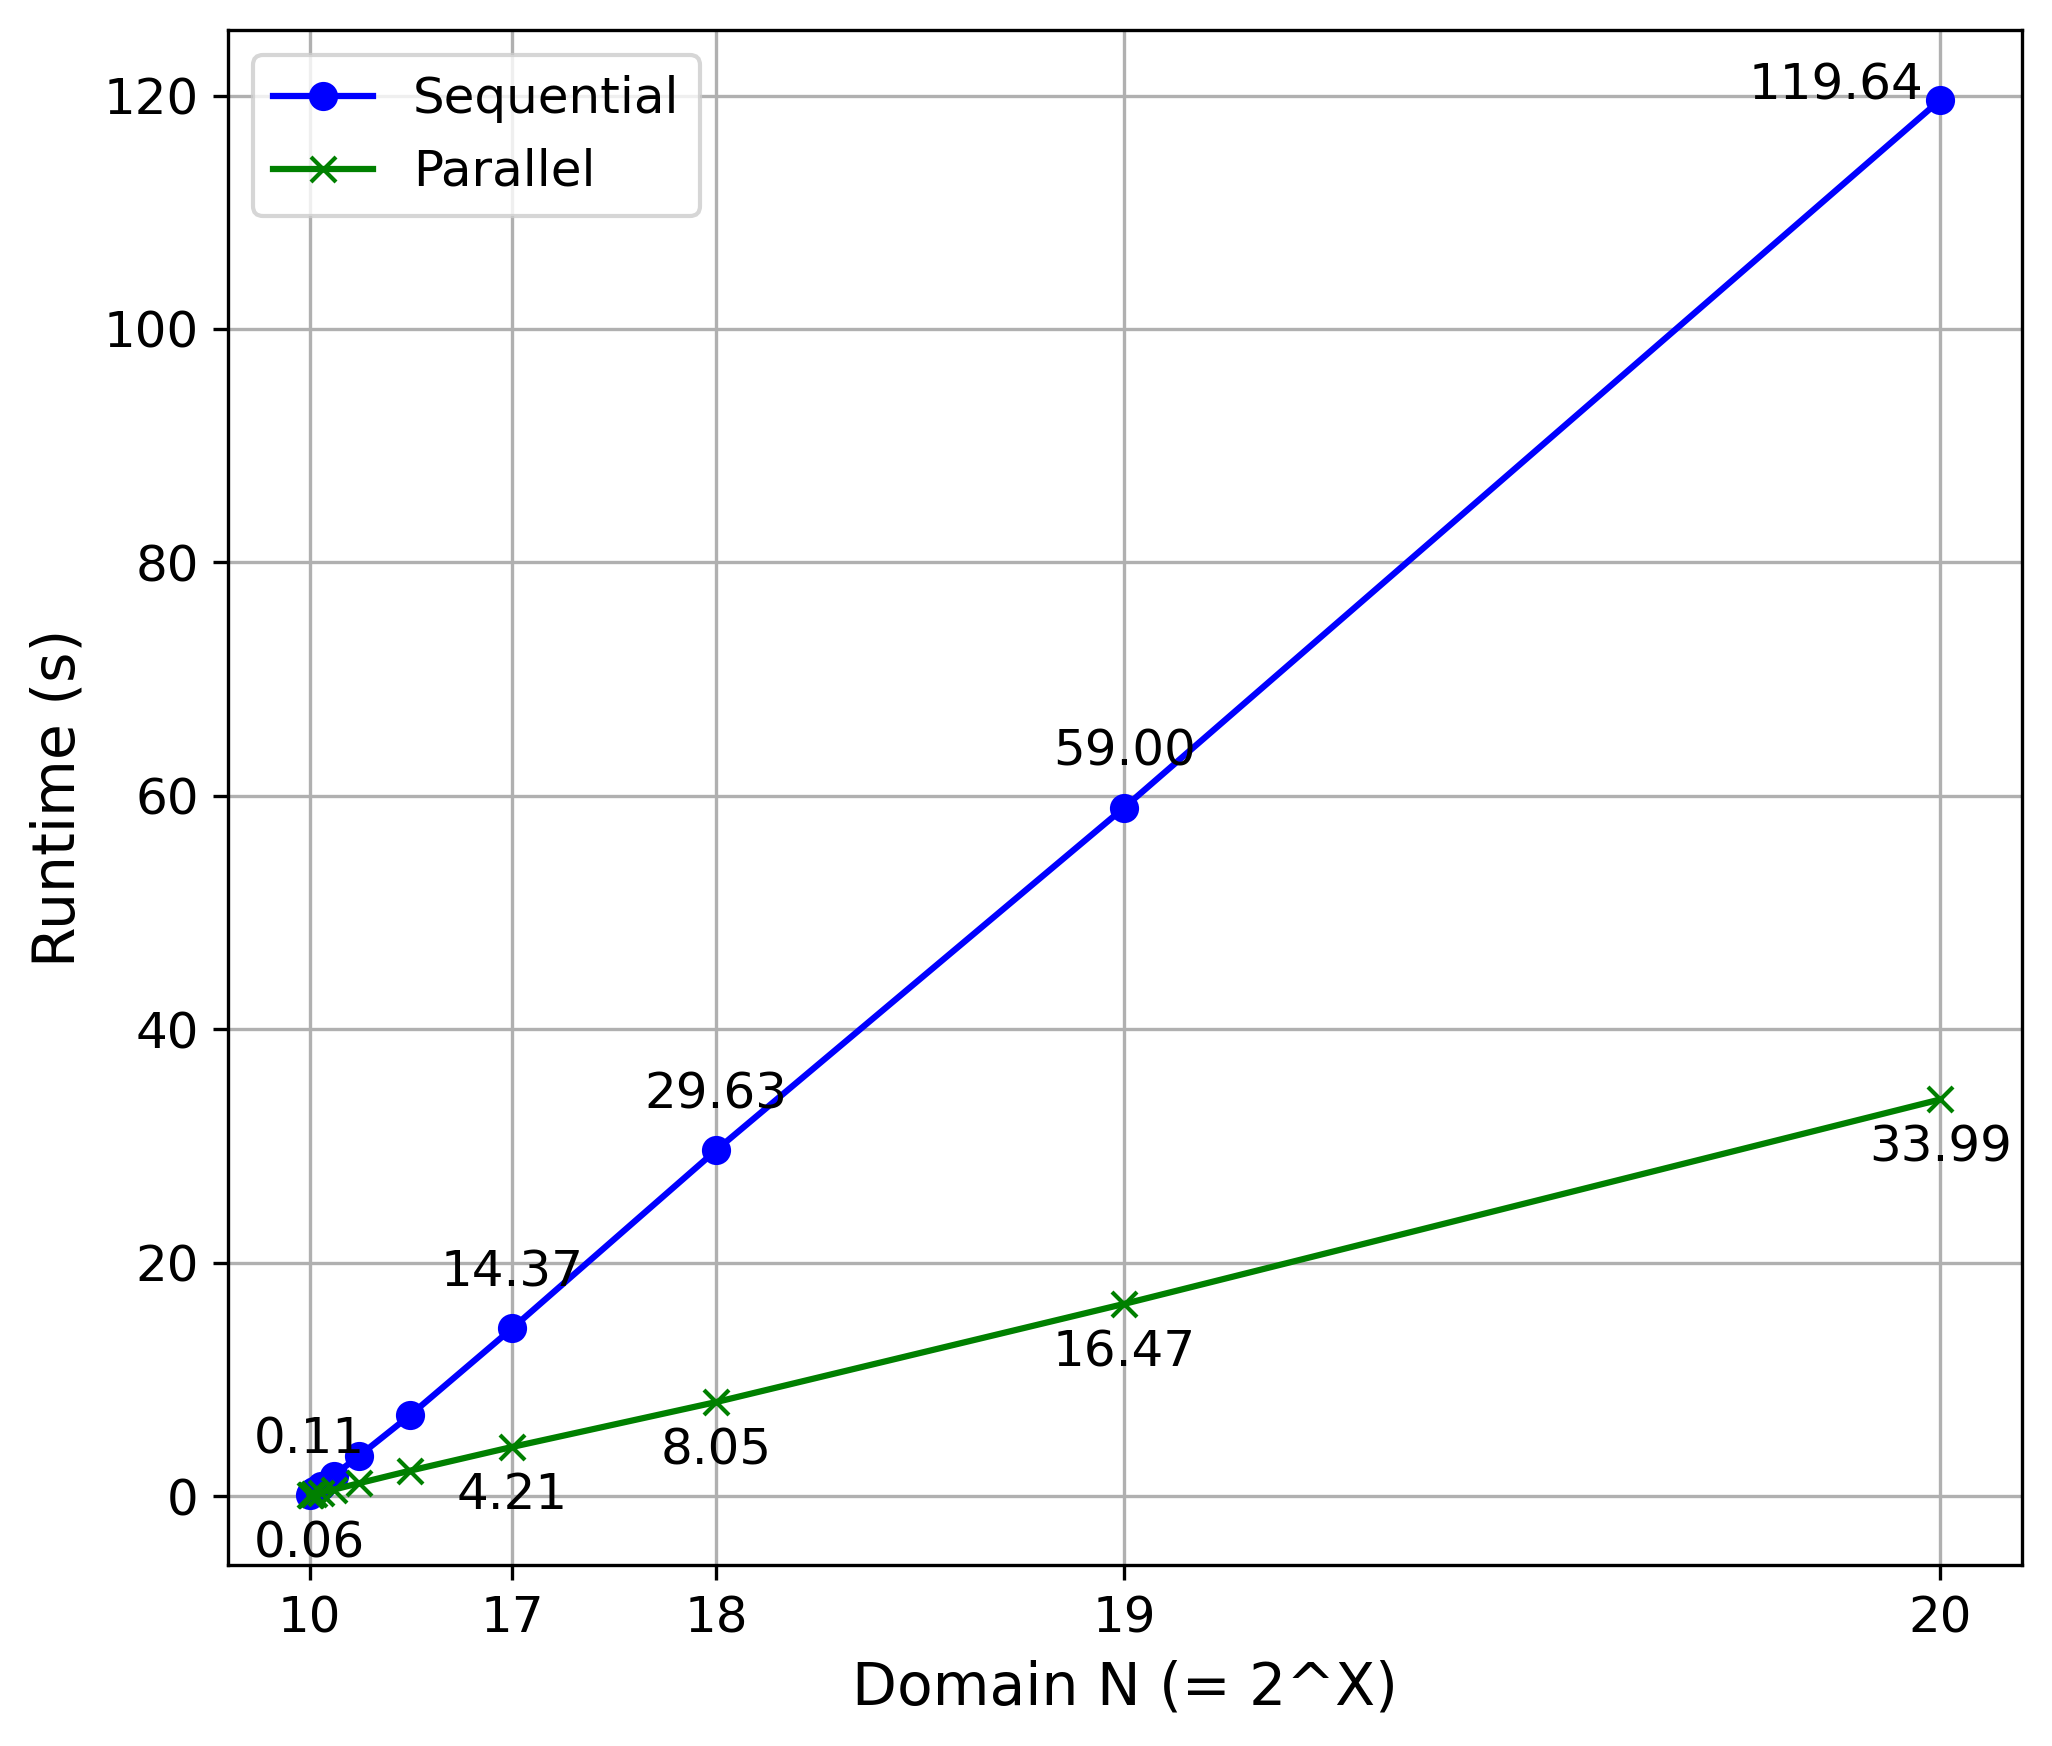
\includegraphics[scale=0.49]{images/plots/full_eval_t16.png}
        \caption{$p=t=16$}
    \end{subfigure}
    \hspace{0em}
    \begin{subfigure}[b]{0.5\textwidth}
        \centering
        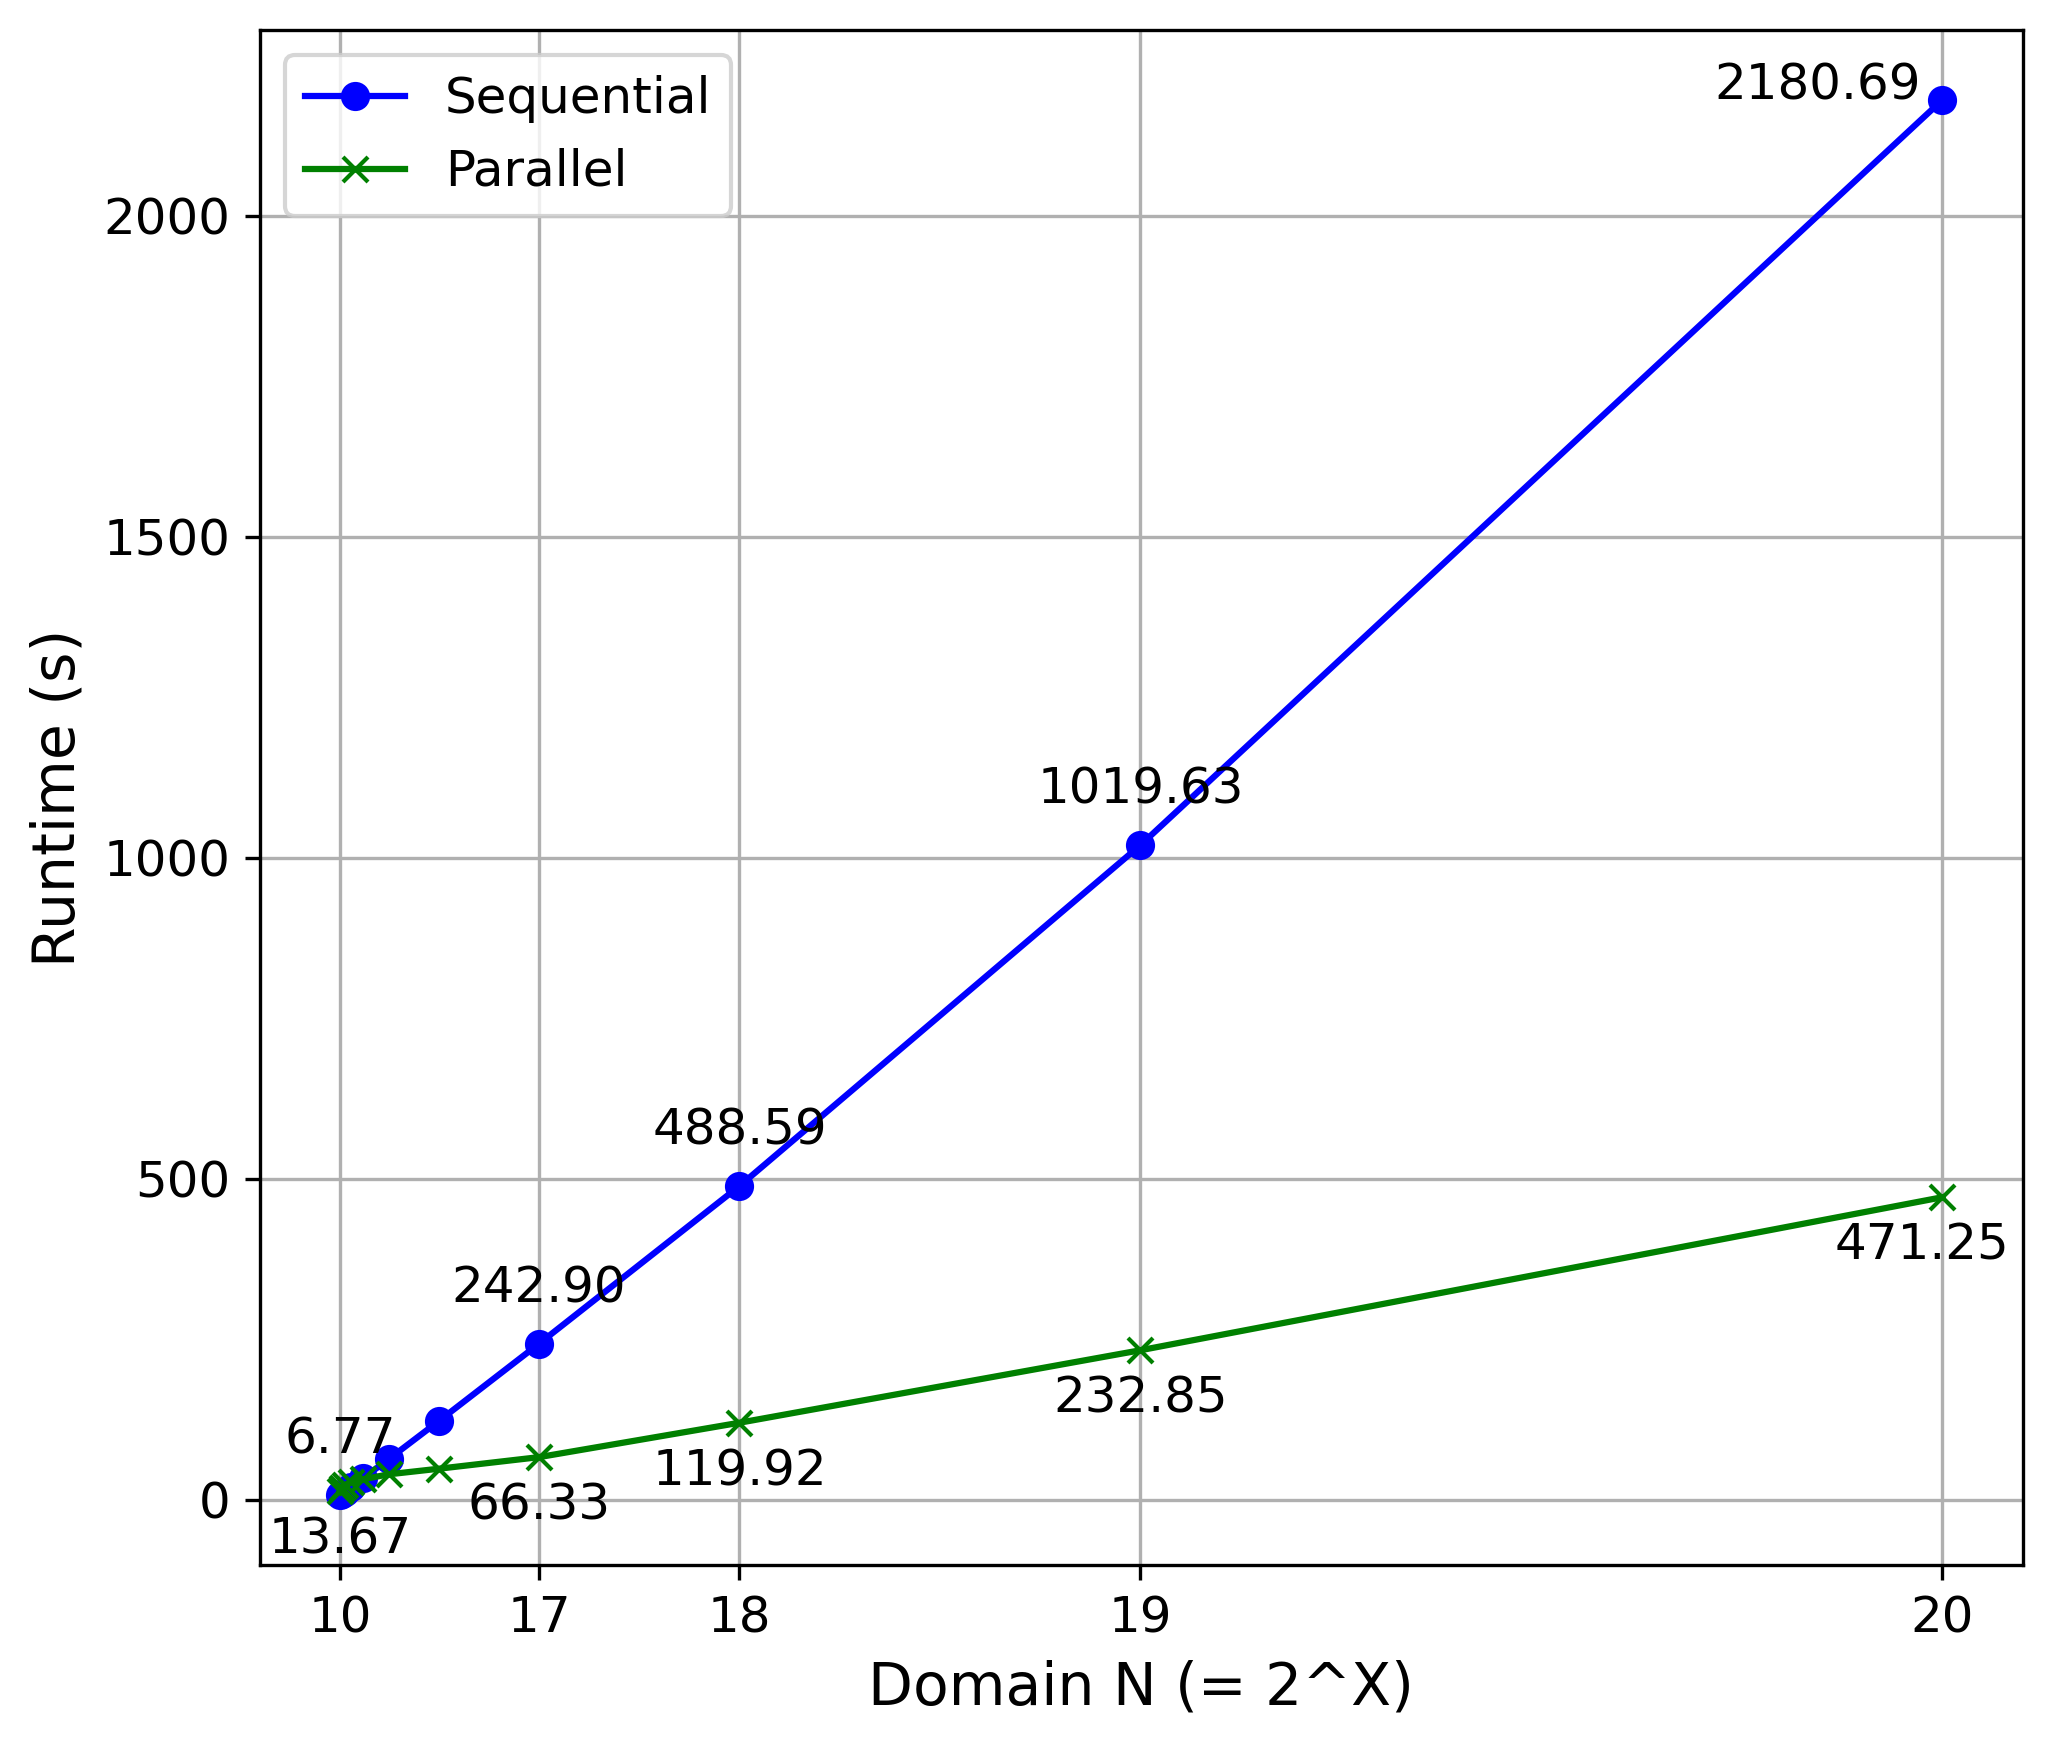
\includegraphics[scale=0.49]{images/plots/full_eval_t256.png}
        \caption{$p =t^2=256$}
    \end{subfigure}
    \label{fig:fullEvalChart}
    \caption{Comparison of sequential and parallel processing of \texttt{DSPF.FullEval}$_N^p$ for $t=16$}
\end{figure}

\subsection{Operations on polynomials of high degree}
In the following, we evaluate the runtime of our polynomial arithmetic implementation, specifically optimized for the PCG use case, where support for high-degree polynomial operations is needed. We evaluate the techniques proposed in Section X for polynomials of up to degree $2^{20}$. These include the Fast Fourier Transform (FFT), sparse polynomial multiplication, and Horner's method. The results indicate that the PCG construction benefits significantly from the strategic use of the techniques used. Without these optimizations, the PCG would not be practical within reasonable time constraints.

\subsubsection{Dense multiplication}
Dense degree $N$ polynomials possess non-zero coefficients for all terms ranging from the constant to $x^N$. As detailed in Section X, their naive multiplication has a computational complexity of $O(N^2)$. On the contrary, the Fast Fourier Transform (FFT) optimizes this operation to $O(N \log N)$. In Figure \ref{fig:polyMultNaiveVsFFT} we present benchmarks for both approaches for $N\in \{2^{10}, ..., 2^{20}\}$. The results confirm the stark difference in scaling: The naive approach demonstrates significantly worse performance compared to the near-linear (or superlinear) runtime achieved by the FFT. The difference between both approaches underlines the importance of using FFT for high-degree polynomial multiplications and, therefore, the PCG implementation.

\begin{figure}[h!]
    \centering
    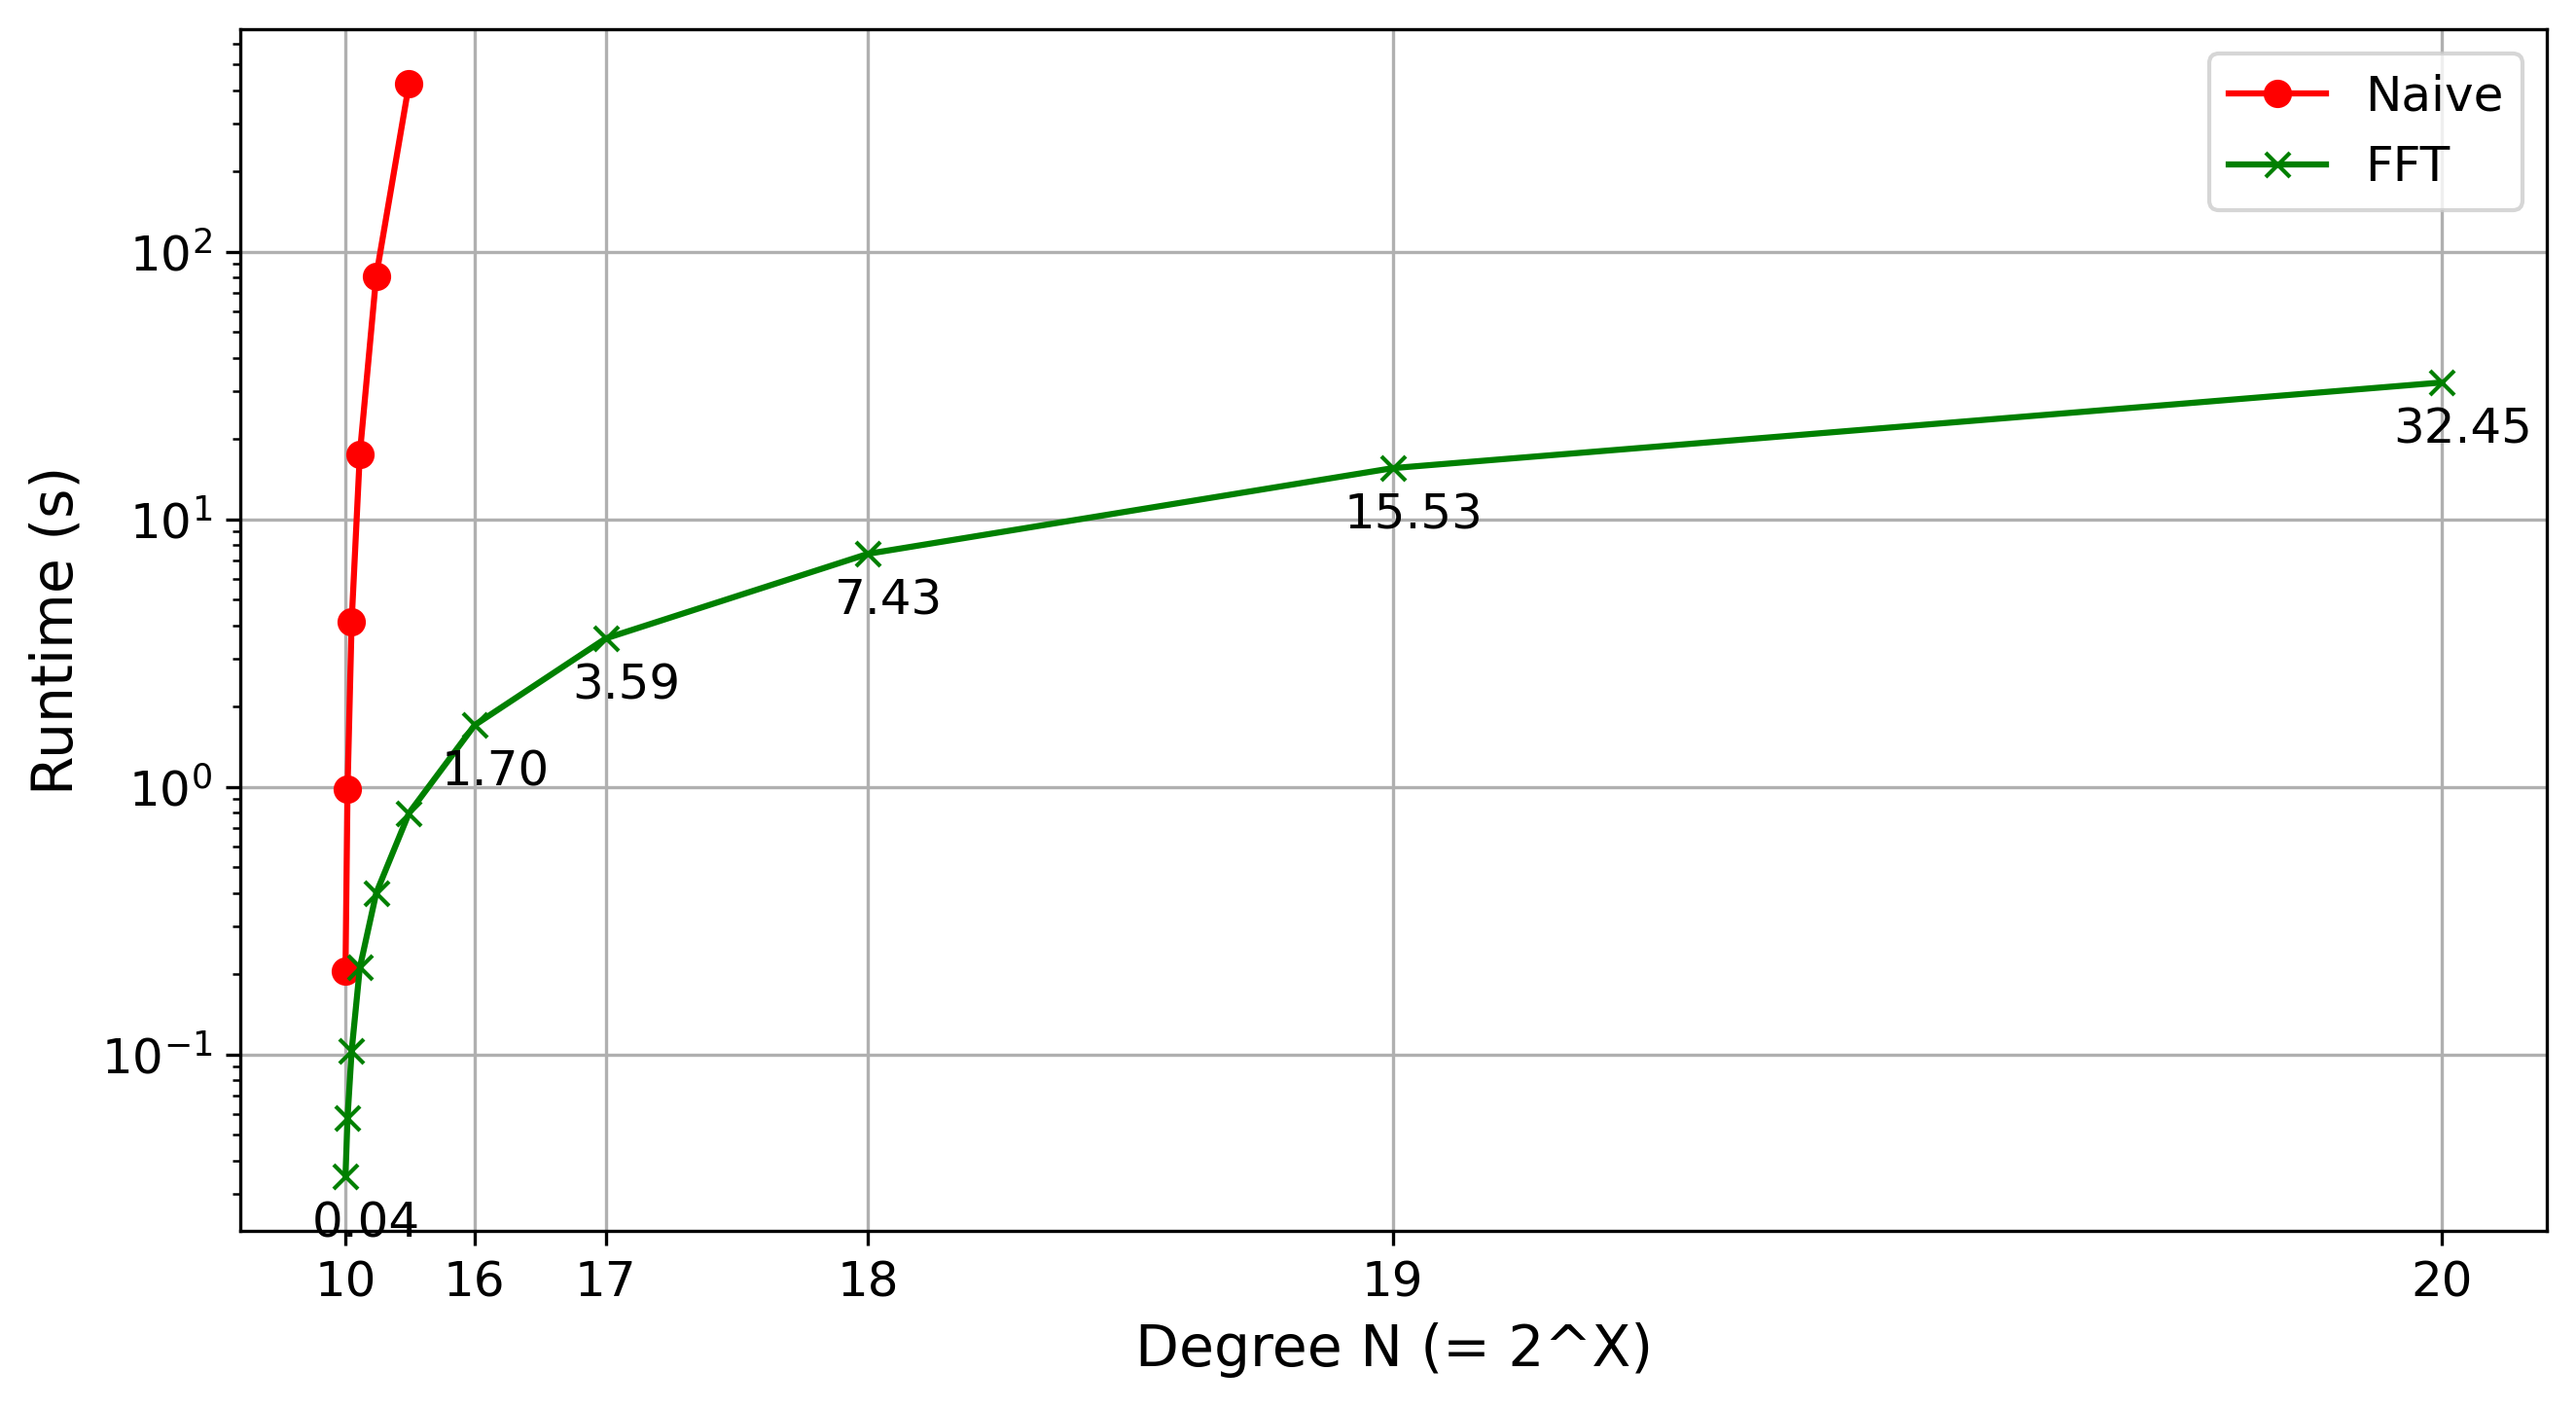
\includegraphics[scale=0.49]{images/plots/poly_mult.png}
    \caption{Comparing approaches to polynomial multiplication of two dense degree $N$ polynomials}
    \label{fig:polyMultNaiveVsFFT}
\end{figure}

\subsubsection{Sparse multiplication}
Sparse polynomials of degree $N$ possess only a few non-zero coefficients within the terms ranging from the constant to $x^N$. In Section X, we proposed that, for certain scenarios, naive multiplication of sparse polynomials could outperform the Fast Fourier Transform (FFT) when zero-coefficient multiplications are efficiently handled. Figure \ref{fig:naiveVsFFTSparsePolys} validates this concept by benchmarking the multiplication of polynomials with varying sparsity for degrees $N=2^{15}$ and $N=2^{18}$. As the complexity of FFT depends solely on the degree of the result, its runtime remains constant for a fixed $N$.  Conversely, the naive approach scales quadratically with sparsity but exhibits significantly lower runtimes for very sparse polynomials. Importantly, the higher the degree $N$, the wider the sparsity range where the naive approach outperforms FFT. In practice, accounting for this in the PCG implementation poses a significant performance increase as the LPN error polynomials are chosen $t$-sparse. When we account for $t=16$ and $N=2^{18}$, a naive multiplication takes only a few ms instead multiple seconds using FFT.

\begin{figure}[h!]
    %\centering
    \hspace{-1em}
    \begin{subfigure}[b]{0.5\textwidth}
        \centering
        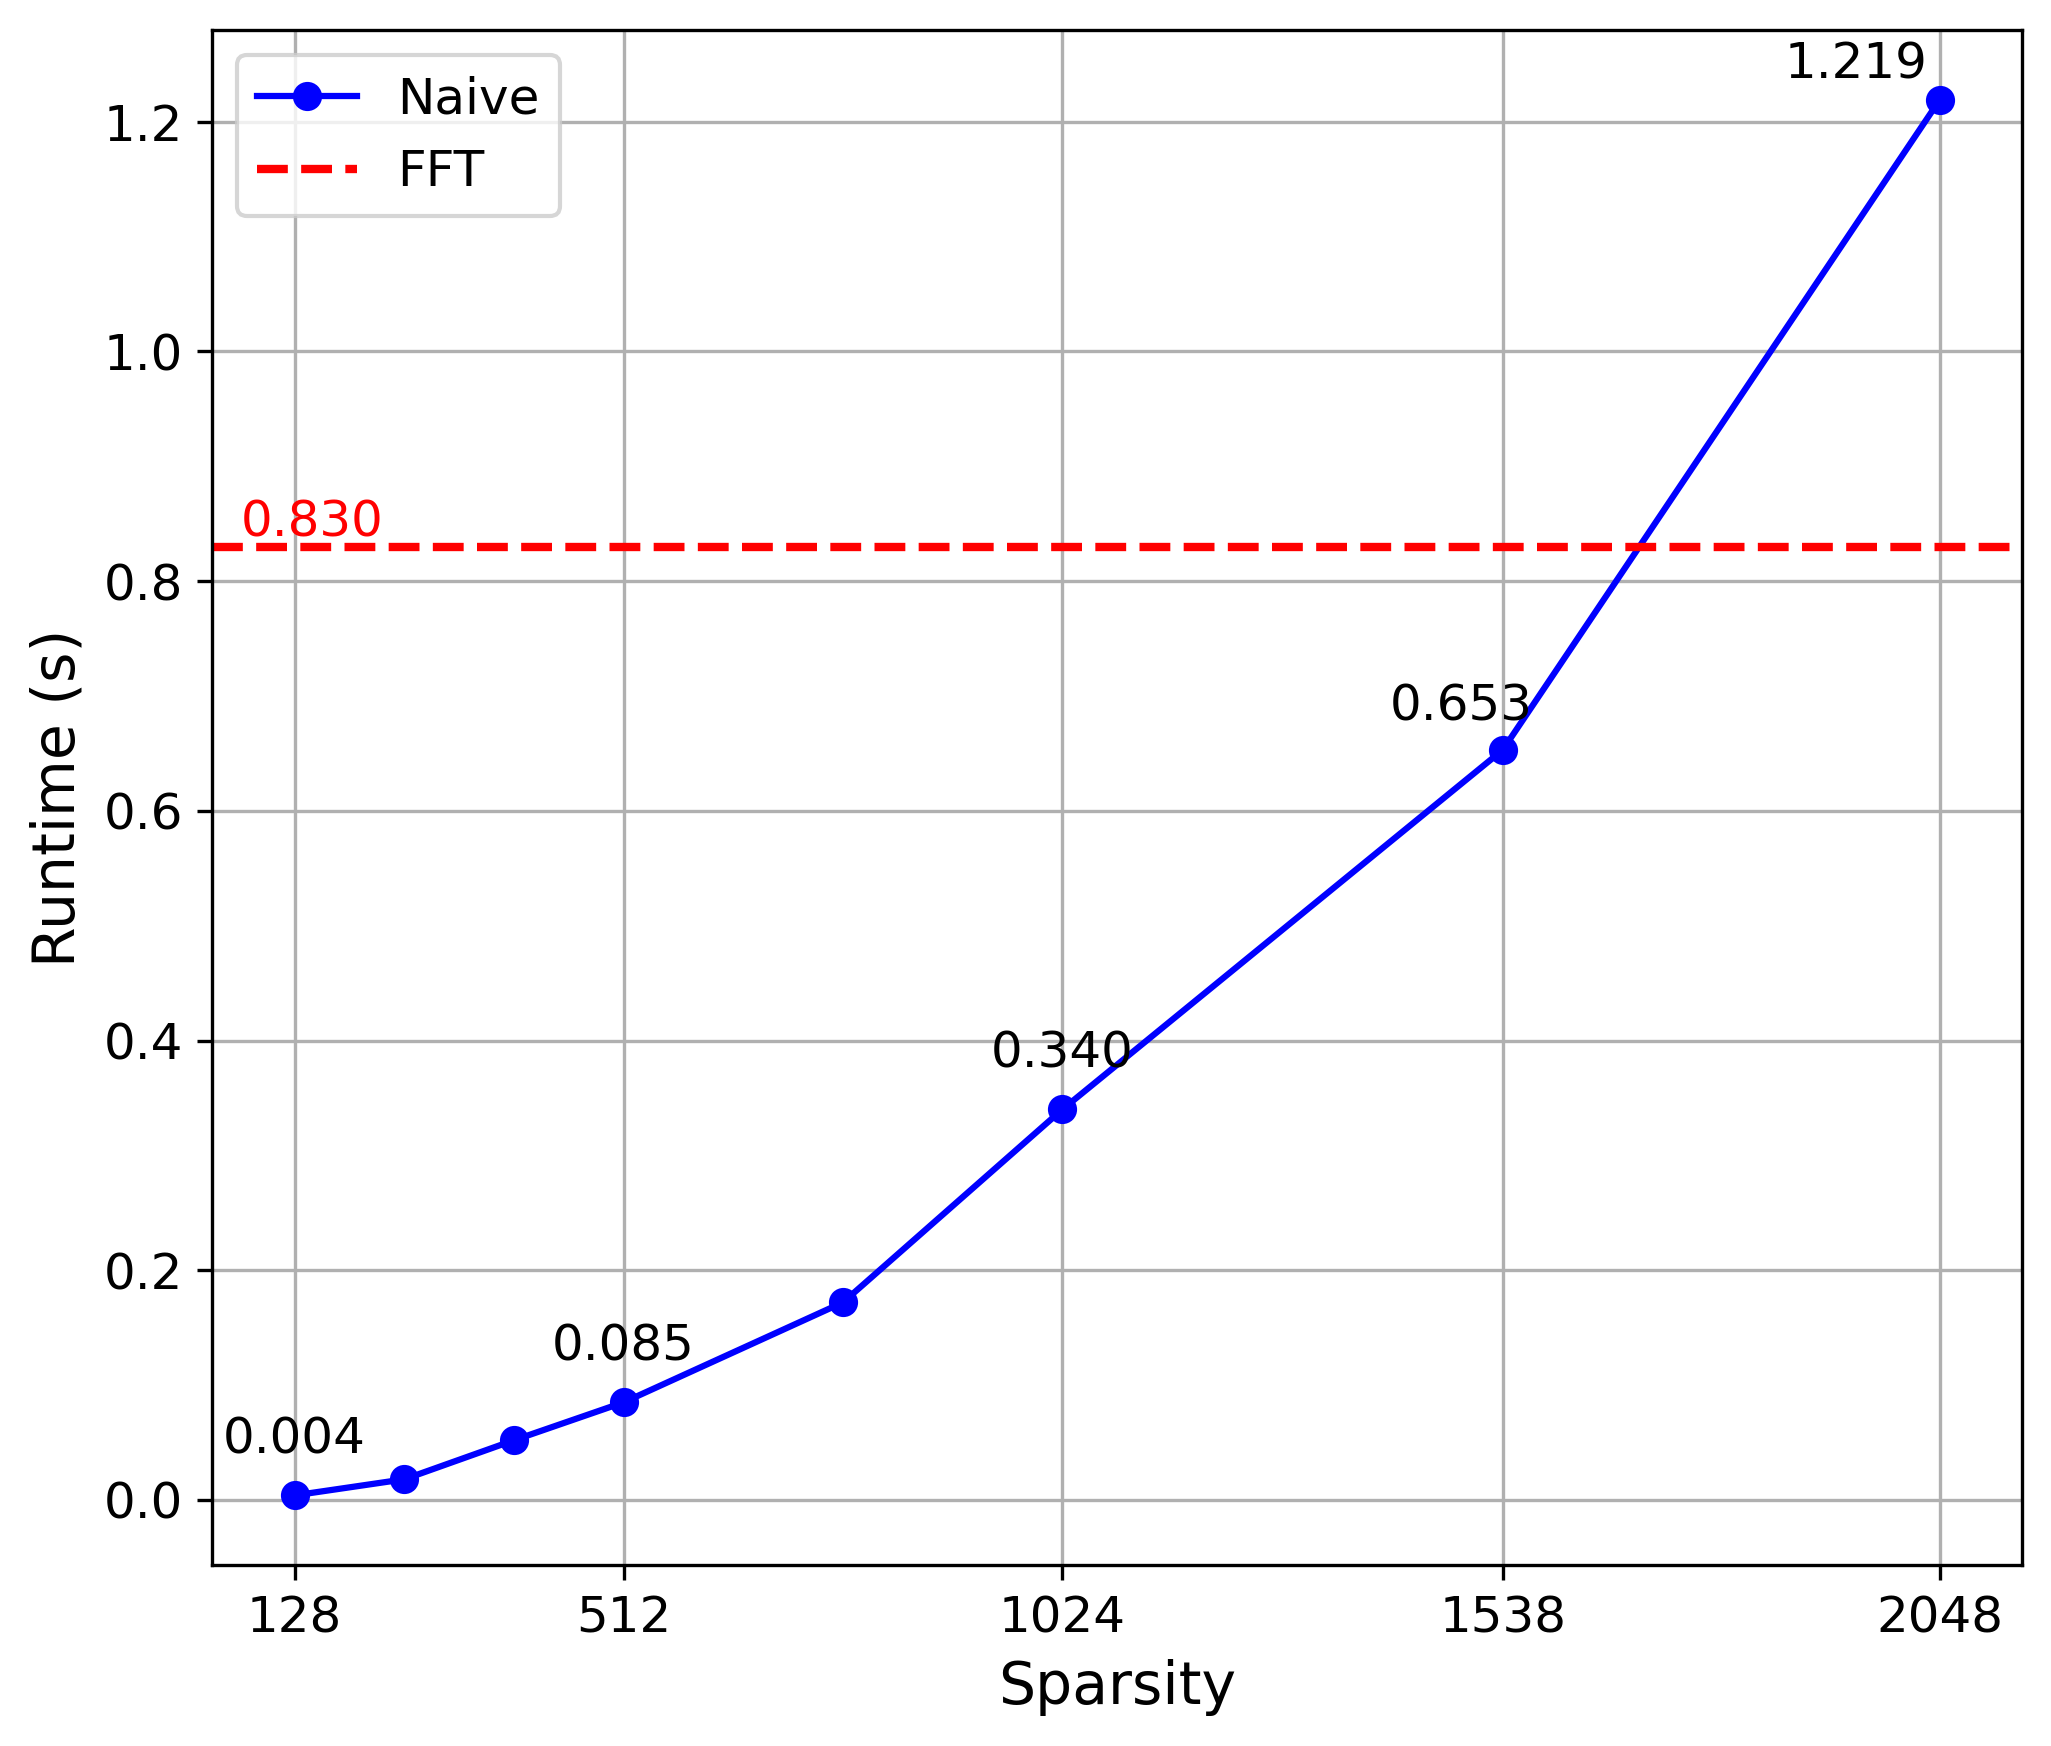
\includegraphics[scale=0.49]{images/plots/poly_mult_sparse_N15.png}
        \caption{$N=2^{15}$}
    \end{subfigure}
    \hspace{0em}
    \begin{subfigure}[b]{0.5\textwidth}
        \centering
        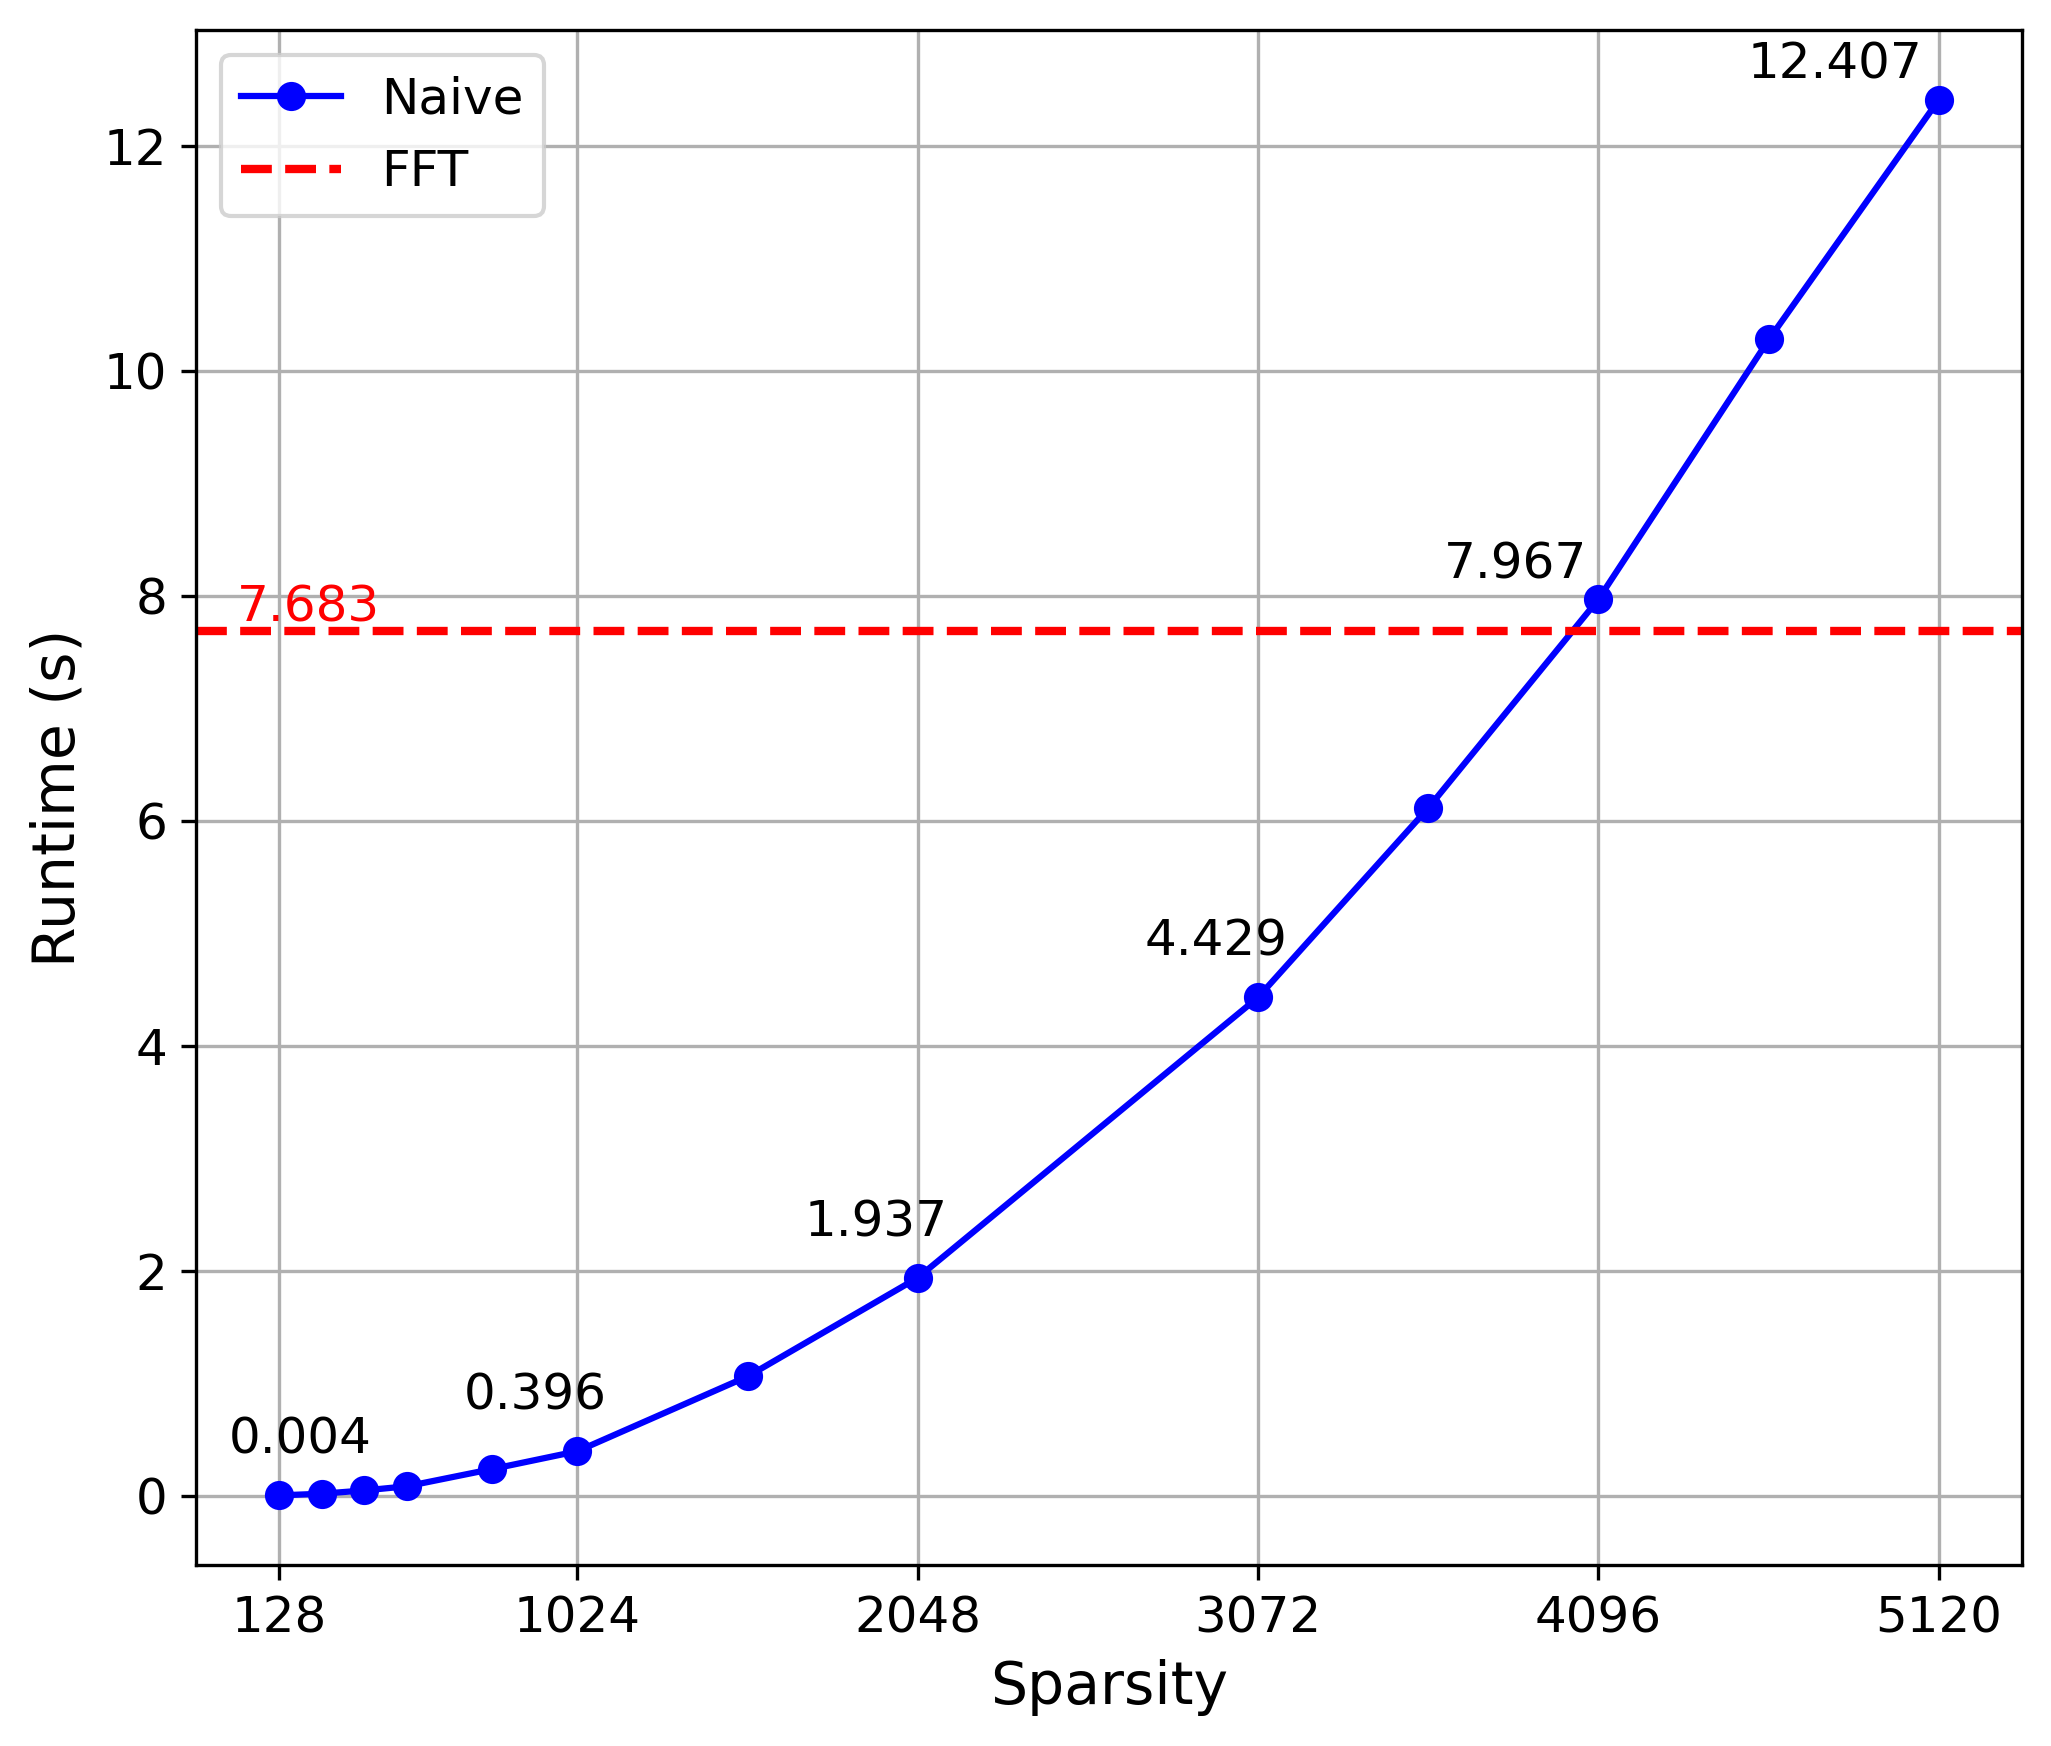
\includegraphics[scale=0.49]{images/plots/poly_mult_sparse_N18.png}
        \caption{$N=2^{18}$}
    \end{subfigure}
    \label{fig:naiveVsFFTSparsePolys}
    \caption{Comparing approaches to polynomial multiplication of two sparse degree $N$ polynomials}
\end{figure}

\subsubsection{Evaluation}
In Section X, we outline how Horner's method optimizes polynomial evaluation to achieve linear $O(N)$ complexity, a significant improvement over the naive quadratic approach. To validate this, we present benchmarks for evaluating polynomials of degree $N \in \{2^{11}, ..., 2^{20}\}$ in Figure \ref{fig:polyEvalBench}. As expected, the naive approach shows worse performance, especially as $N$ increases. Horner's method demonstrates a clear linear runtime increase, enabling the evaluation of a degree $N=2^{20}$ polynomial at a specific position in approximately 165ms. However, after PCG expansion, $N$ individual position needs to be evaluated on (multiple) polynomials to extract all (V)OLE correlations. This underscores the importance of polynomial evaluation for the PCG.
\\\\
\textbf{Parallelization.} To address a potential bottleneck, we explore parallelization. Unlike parallelizing multiple evaluations, our strategy directly enhances performance for single-point evaluations – potentially beneficial if storage complexity is a concern and parties split the ring on demand (Section X). Our parallelized implementation of Horner's method achieves a near-10x speedup, demonstrating good hardware utilization. This reduces the evaluation time for a degree $N=2^{20}$ polynomial to 17.7ms, down from 165ms.

\begin{figure}[h!]
    \centering
    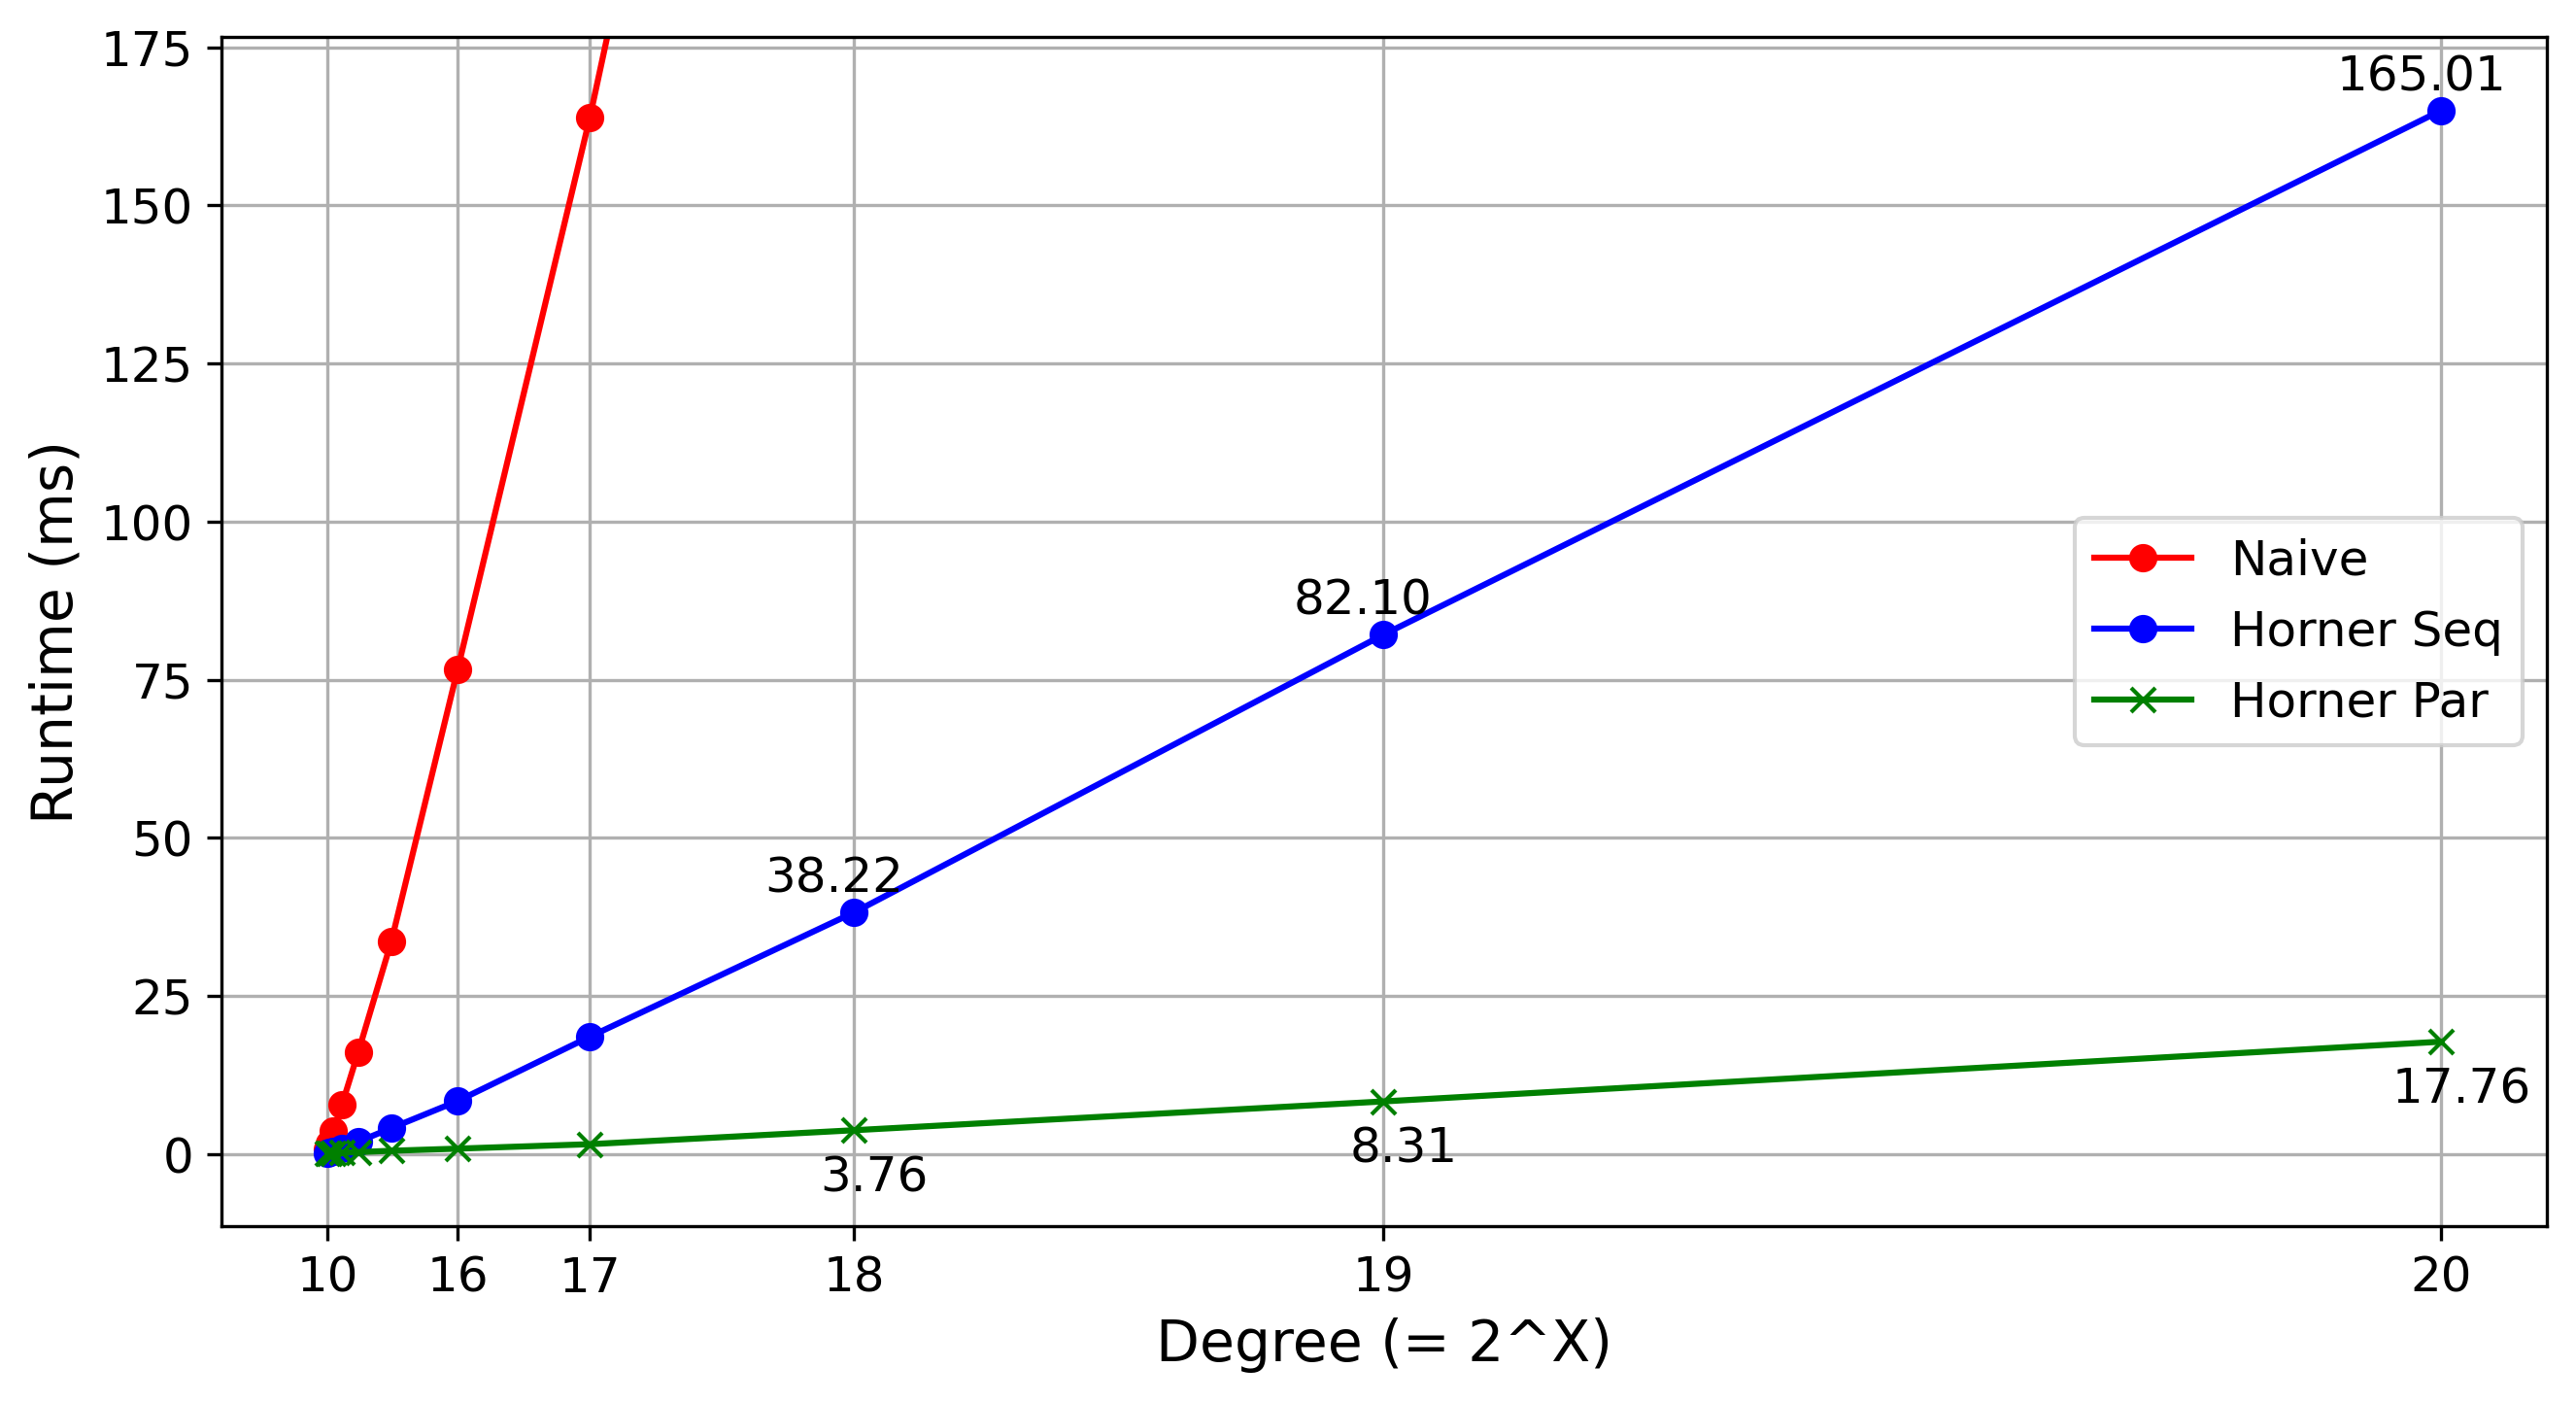
\includegraphics[scale=0.49]{images/plots/poly_eval.png}
    \caption{Comparing approaches to polynomial evaluation of two dense degree $N$ polynomials}
    \label{fig:polyEvalBench}
\end{figure}


\subsection{Computing roots of unity}
In the following, we evaluate our implementation for computing all roots of unity for the $2N$-th cyclotomic polynomial. As outlined in Section X, we implemented two approaches: the naive method directly iterates over Equation X to generate all roots of unity, while the optimized approach leverages a Horner inspired technique to reuse exponentiations for improved efficiency. The benchmarks for $N=\{2^{15}, ..., 2^{20}\}$ (Figure X) show that the optimized approach scales linearly. This is beneficial for PCG construction, as it does not negatively affect the time required per (V)OLE correlation for higher PCG domains. Note also that we achieve a significant performance improvement of about 11x over the naive method.

\begin{figure}[h!]
    \centering
    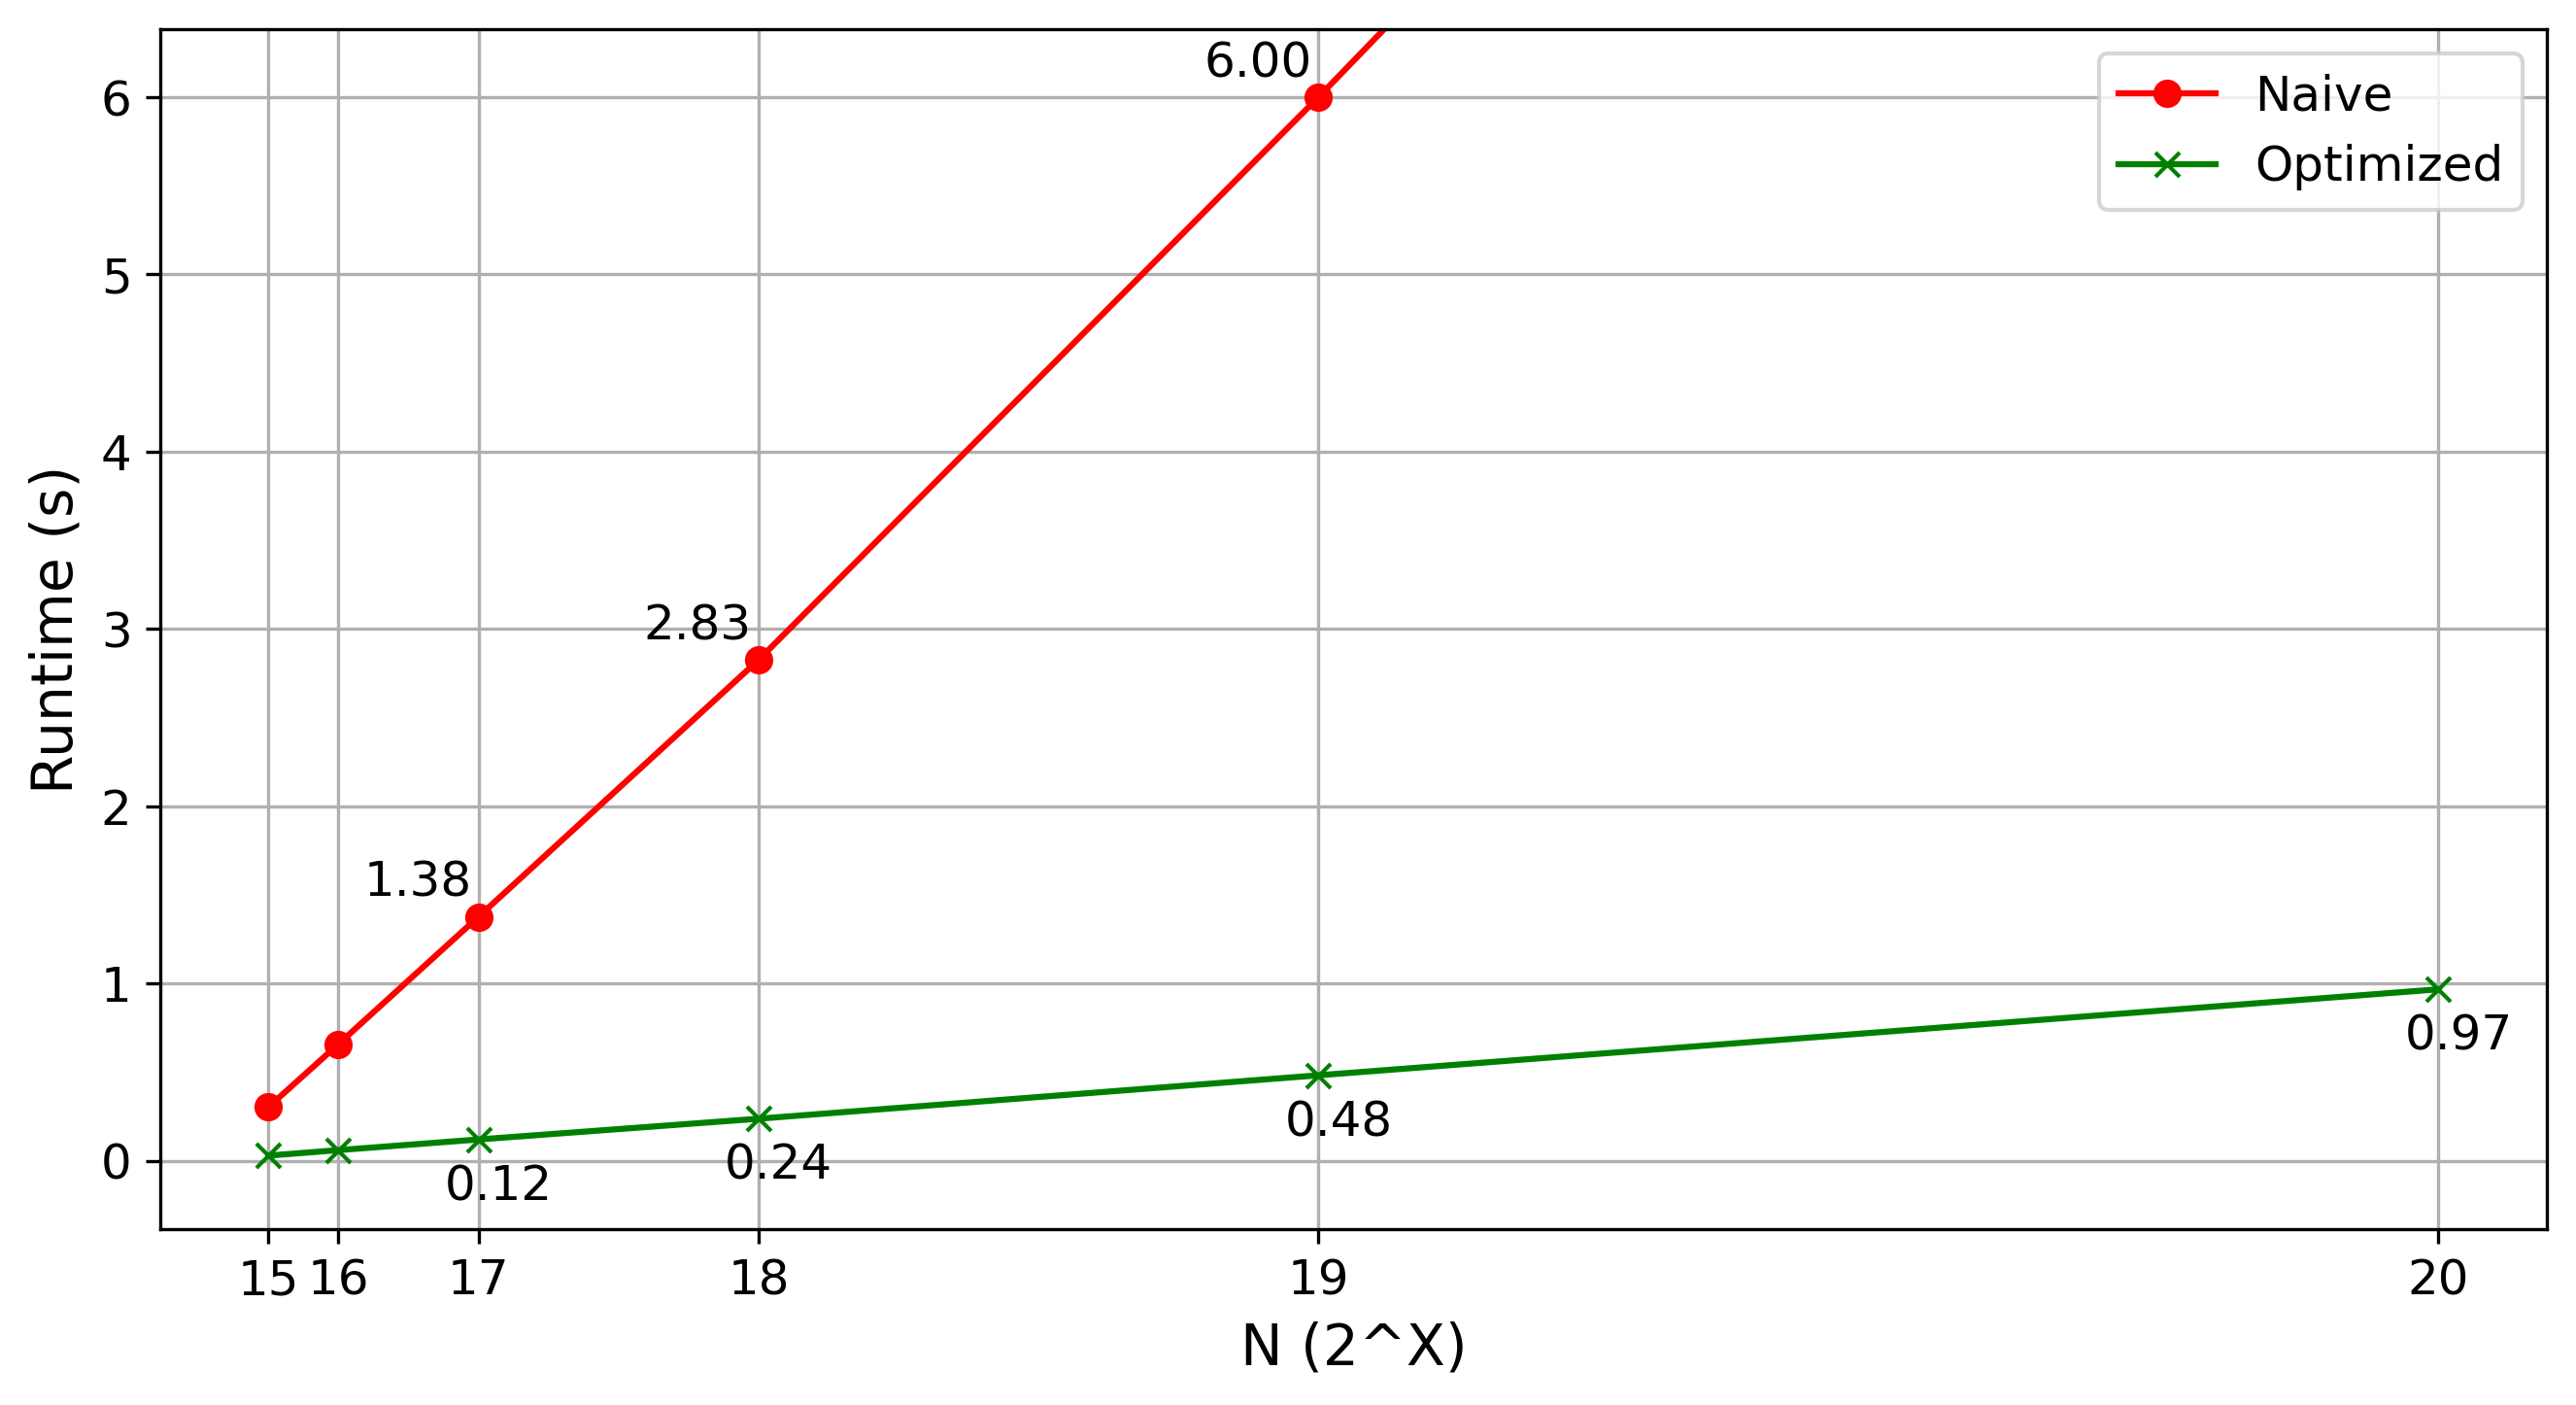
\includegraphics[scale=0.49]{images/plots/gen_roots.png}
    \caption{Comparing approaches to generate all \textit{roots of unity} for the $2N$-th cyclotomic polynomial}
\end{figure}


\section{PCG construction}
In this section, we evaluate the PCG construction of Section X for different domains $N$. We choose the LPN parameters to be $(c,t)=(4,16)$ which achieve $128$-bit security, as shown by Boyle et al. \cite{boyle2020efficient}. Benchmarks are conducted for domain sizes $N\in\{2^{10}, ..., 2^{18}\}$. 

\subsection{Generation}
Figure \ref{fig:ComparingPCGGeneration} reveals the runtime efficiency of PCG seed generation, particularly when using a trusted dealer. This contrasts with the higher overhead of distributed generation algorithms, which are not part of this work. It is worth noting that distributed generation alternatives exist, but they introduce significant performance tradeoffs.
\\\\
The VOLE construction requires four calls to \texttt{DSPF$^{t}_{N}$.FullEval}. With $t=16$, this translates into 64 underlying DPF calculations (see Section X for more context). On the contrary, the OLE construction performs 16 calls to \texttt{DSPF$^{t^2}_{2N}$.FullEval}, demanding a significantly higher 4096 DPF computations. This 64x increase in DPFs aligns well with the benchmark results. For $N=2^{18}$, the OLE runtime of 0.44s is approximately 68 times longer than the VOLE's 0.0064s. 

\begin{figure}[h!]
    \centering
    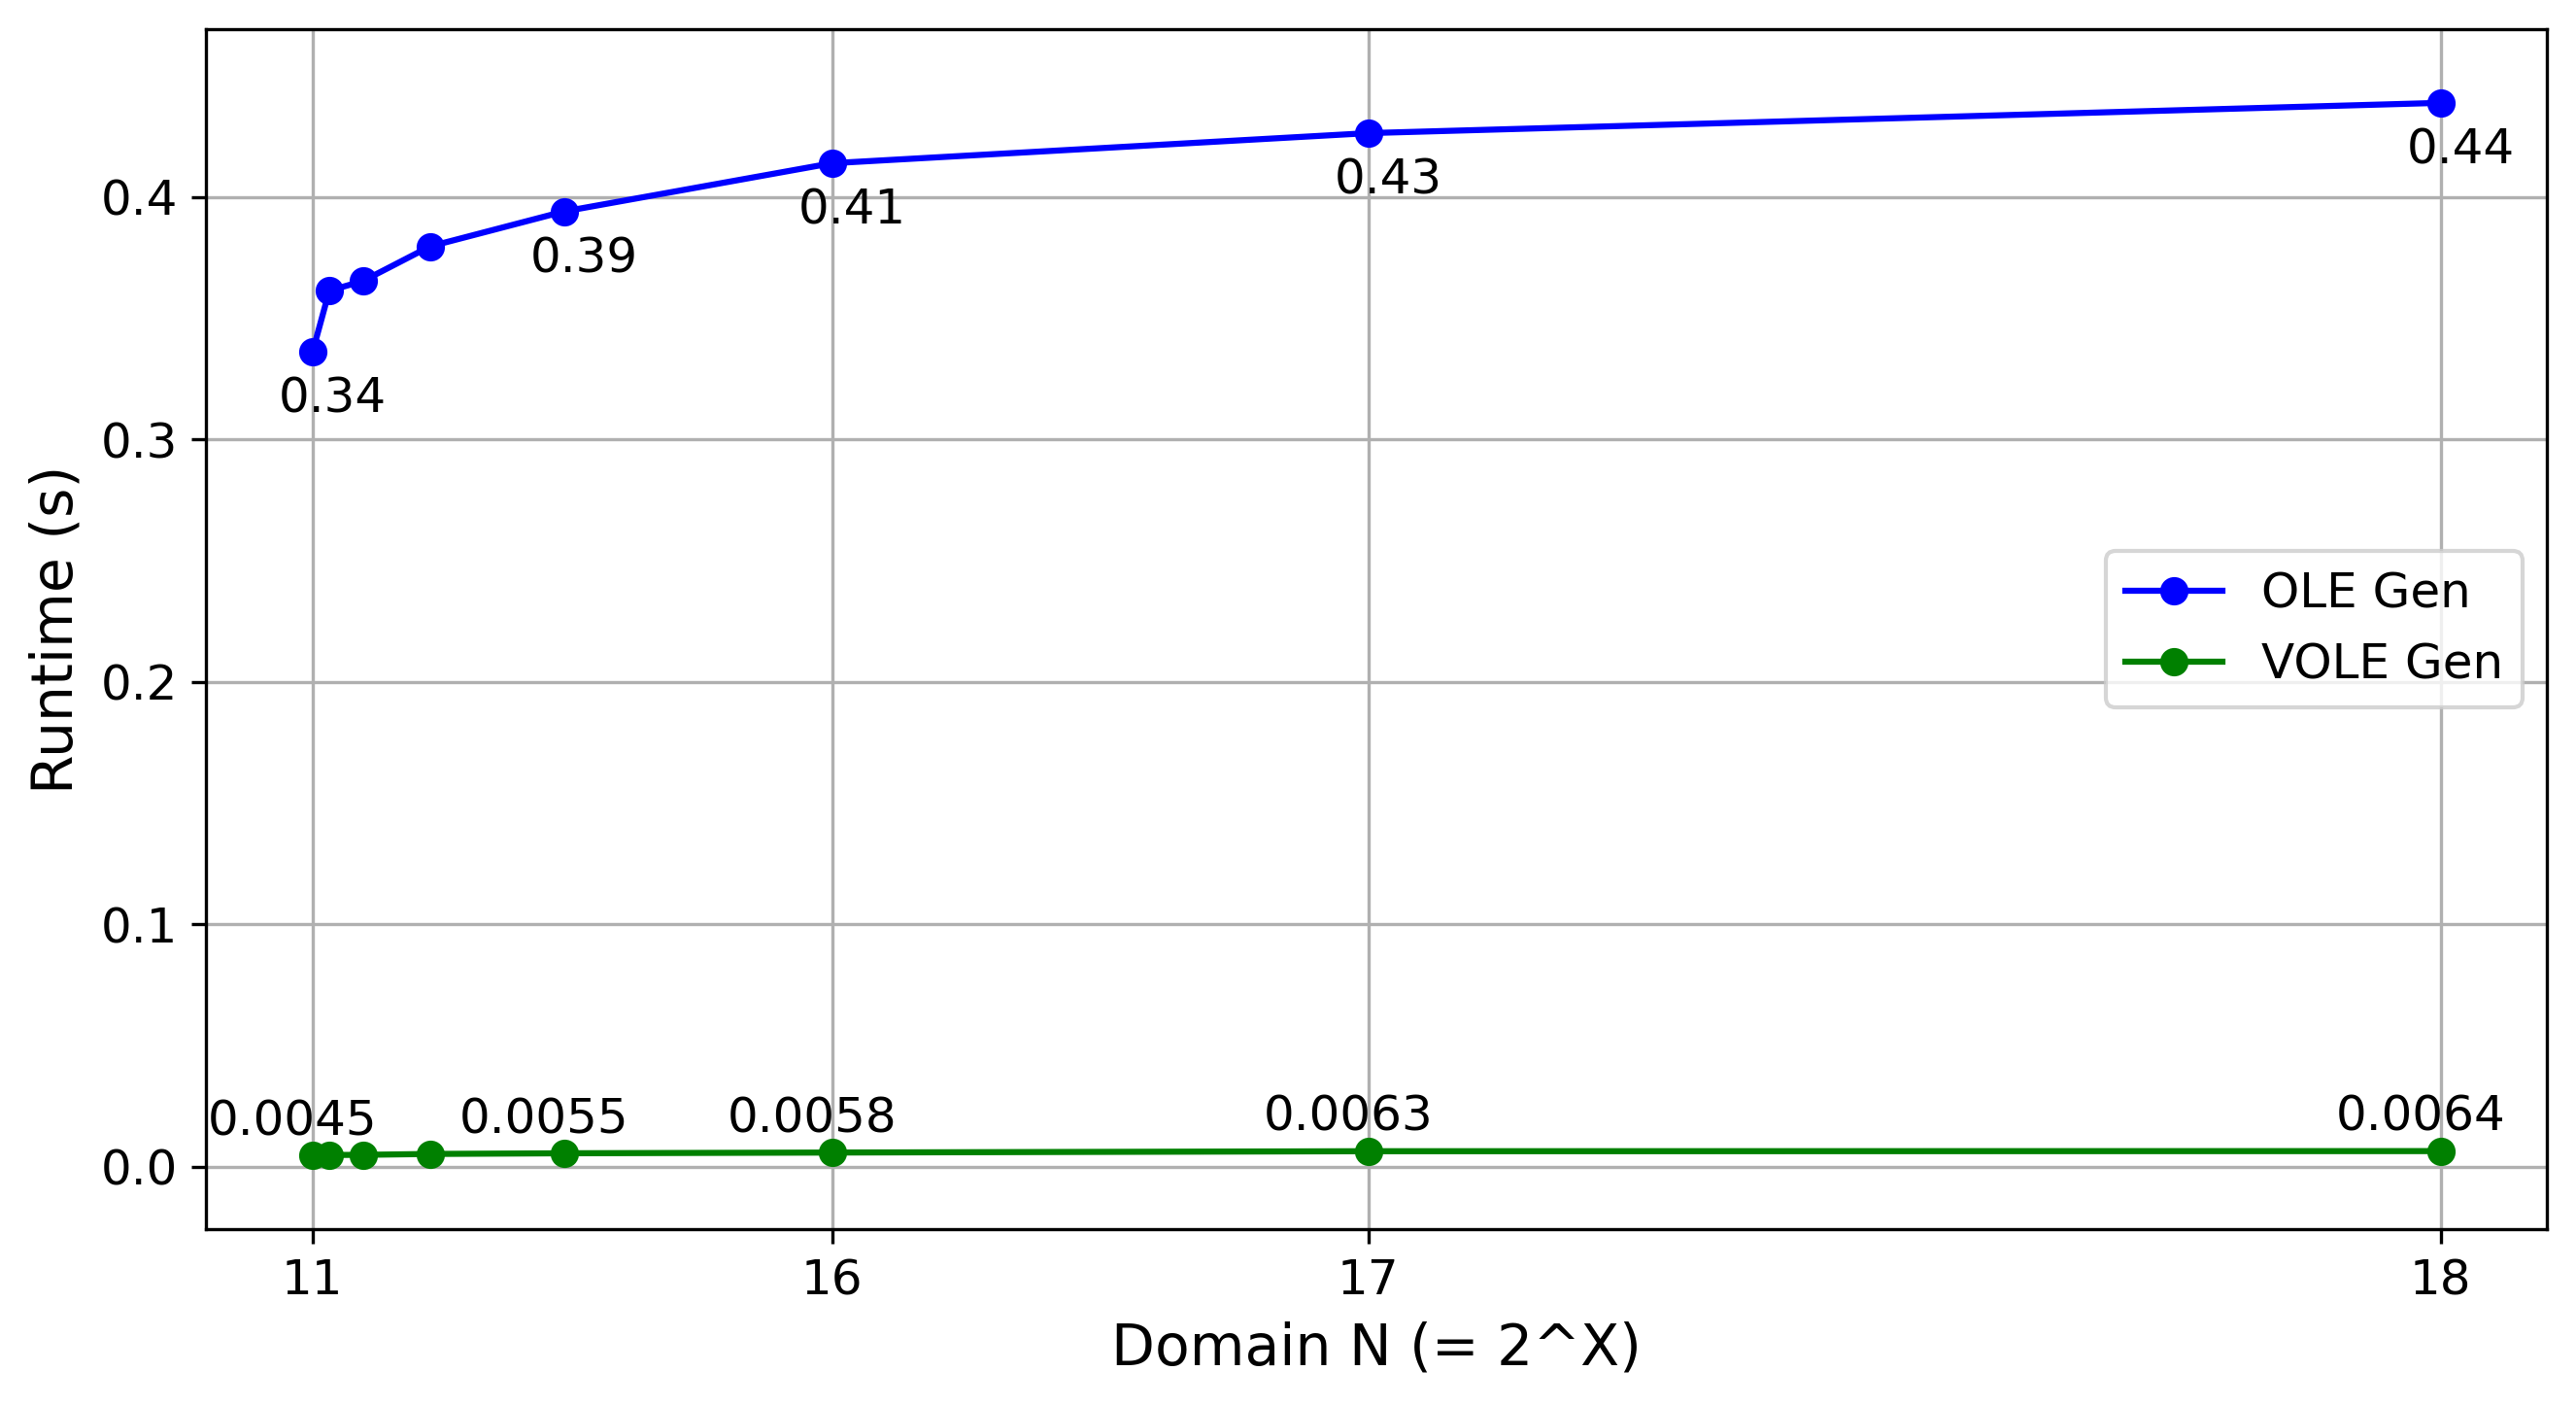
\includegraphics[scale=0.49]{images/plots/pcg_gen.png}
    \caption{Comparing the PCG expansion OLE and VOLE}
    \label{fig:ComparingPCGGeneration}
\end{figure}

Interestingly, the domain size $N$ has a relatively minor impact on generation time. This comes from the tree-based approach used within the underlying DPFs. Doubling $N$ leads to a roughly constant increase in operations (proportional to $t$ or $t^2$), due to the fixed value of $t$. 

\subsection{Expansion}
We present the runtimes of the PCG constructions relative to the amount of (V)OLE correlation they generate in Figure \ref{fig:ComparingPCGExpansion}. This figure also separately visualizes the added cost of extracting correlations (splitting the ring elements) via polynomial evaluation on a root of unity. Observe the superlinear scaling for both OLE and VOLE constructions with respect to $N$. As discussed previously, this primarily stems from the superlinear nature of polynomial multiplication using FFT, despite achieving linearity in other building blocks. It is worth emphasizing that compared to the expansion itself, our optimized computation of roots of unity adds negligible overhead. For example, with $N=2^{18}$, this step adds only 0.24 ms per correlation.

\begin{figure}[h!]
    \centering
    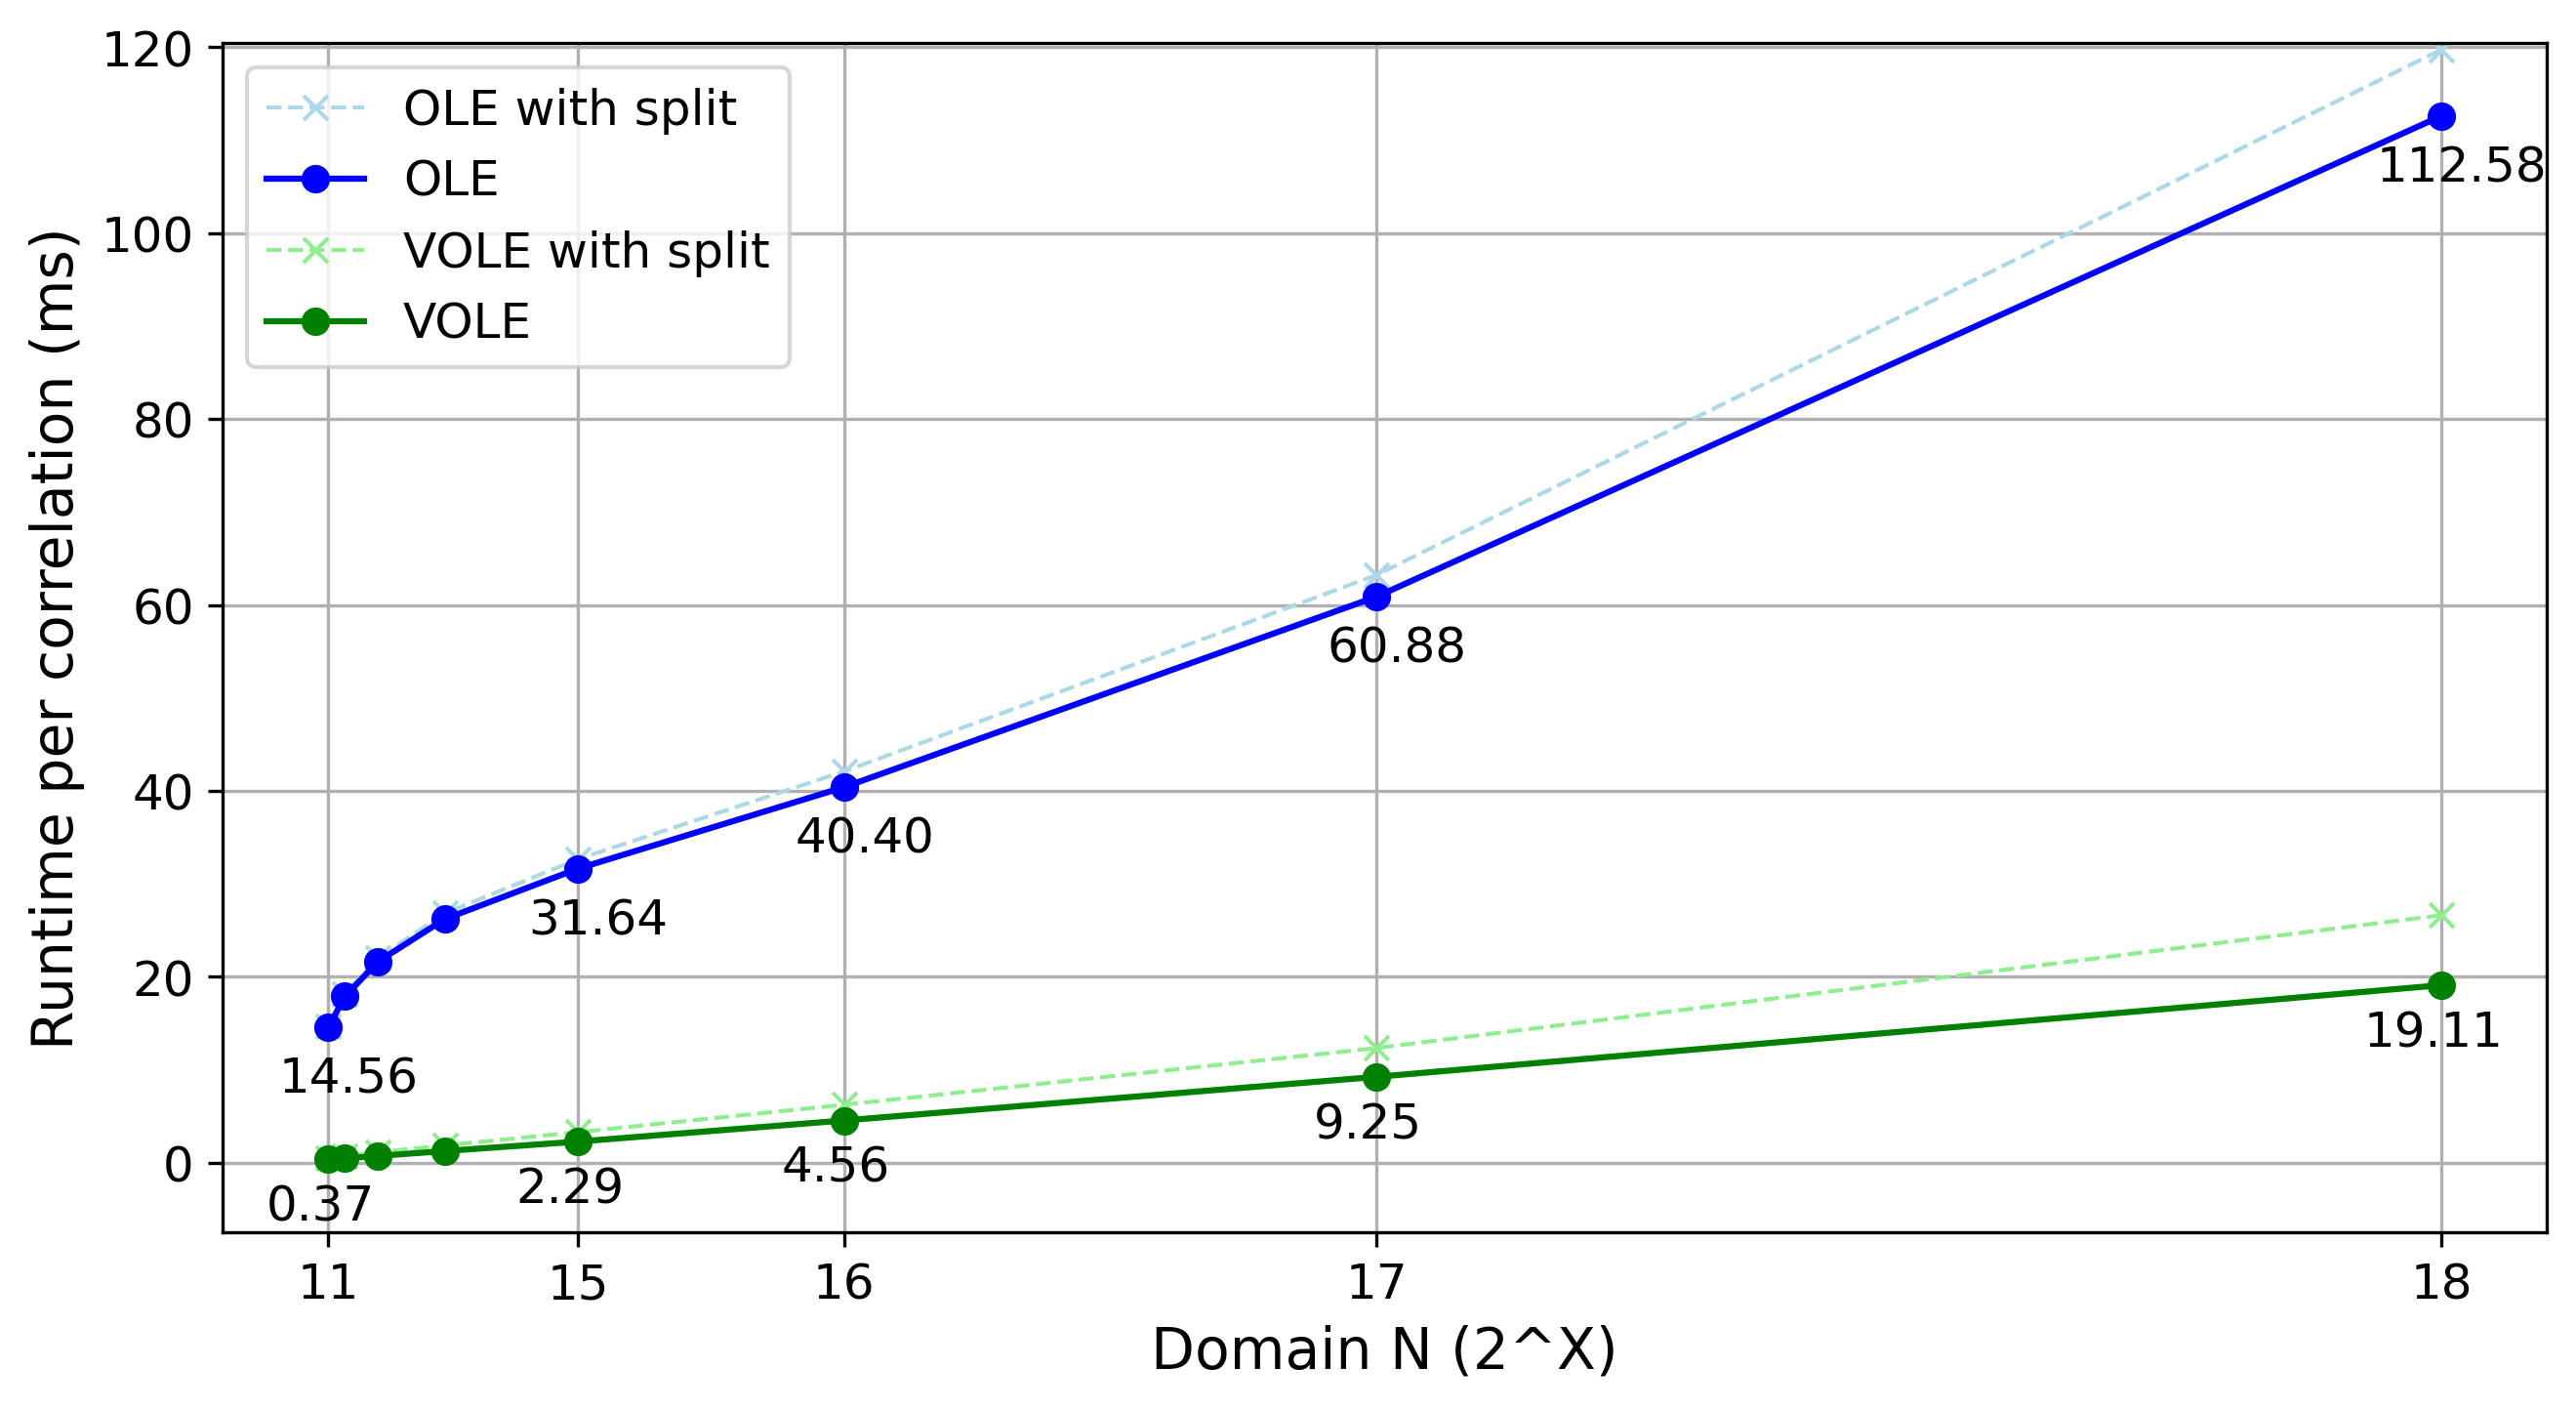
\includegraphics[scale=0.49]{images/plots/pcg_eval.png}
    \caption{Runtime comparison of the PCG expansion for OLE and VOLE over $N$}
    \label{fig:ComparingPCGExpansion}
\end{figure}

We observe a nearly exponential runtime increase in OLE construction for small $N$, transitioning to the expected superlinear increase as $N$ grows. We identify this behavior as an effect of the parallelization overhead that dominates in small domains. As $N$ increases, the parallelization setup cost amortizes, revealing the construction's expected superlinear runtime. The same applies to the VOLE construction, but is less visible due to the figures scaling. Notably, the VOLE construction scales more favorably than OLE construction, exhibiting a near-linear runtime. Several factors explain this:

\begin{itemize}
    \item \textbf{Reduced Multiplications:} With $c=4$, the VOLE construction requires only $8$ polynomial multiplications compared to OLE's $24$. Since multiplications (via FFT) drive the superlinear runtime, their reduced usage in the VOLE construction yields a runtime closer to the complexity of other primitives.
    
    \item \textbf{Lower Degrees:} The multiplications of the VOLE construction operate on degree-$N$ polynomials, while a significant portion of OLE constructions multiplications involve degree-$2N$ polynomials. As FFT complexity becomes closer to linear for smaller degrees, this further reduces its overall impact in the VOLE construction.
    
    \item \textbf{Exploiting Sparsity:} The VOLE construction involves more sparse polynomial multiplications. Here, our optimized approach strategically selects the more efficient naive method, further improving performance.
\end{itemize}

\textbf{Splitting the Ring:} Note that the (V)OLE constructions do not include the splitting of the ring elements. However, since this is a crucial practical step, we include the overhead it introduces in Figure \ref{fig:ComparingPCGExpansion}. Our parallelized optimizations of Horner's method for polynomial evaluation yield noticeable benefits, resulting in a moderate overhead for the constructions. At $N=2^{18}$, the increase is 39.35\% for VOLE and only 6.34\% for OLE. While the absolute runtime for this operation is identical in both cases, the proportional increase is higher for the VOLE construction due to its lower overall runtime. Therefore, we find that further optimizations would be valuable, particularly to reduce the overhead associated with ring splitting in the VOLE case.
\\\\
\textbf{Profiling:} Our analysis suggests in several passages that FFT-based polynomial multiplications are the primary runtime bottleneck in PCG constructions. Although this is the case, we found that the impact of the FFT varies with $N$ and differs between OLE and VOLE. To validate this, we analyze the runtime distribution between generating ring elements (where FFT is used) and the cost of fully evaluating DSPFs in Figure \ref{fig:runtimeAllocationComparision}. We observe that for the OLE construction, the superlinarity of the FFT becomes dominant only for larger $N$. This is also due to the fact that the runtime required for the (large) DSPF full domain evaluations is quite high to begin with, which is less the case for the smaller DSPF domains in the VOLE case (a precise comparison is given in the following paragraph). This is also the reason why the FFT is more dominant for smaller $N$ in the VOLE construction. Recall from section \ref{subsec:evalDspfFullDomain} that the advantage of parallelizing the full domain evaluation for the OLE case increases with larger $N$ compared to the VOLE case. This can be clearly seen here, as the increase in the dominance of the FFT increases steadily for OLE, but flattens out for VOLE. Ultimately, the superlinear nature of the FFT implies that its runtime share will approach 100\% in both constructions as $N$ continues to increase.

\begin{figure}[h!]
    %\centering
    \hspace{-1em}
    \begin{subfigure}[b]{0.5\textwidth}
        \centering
        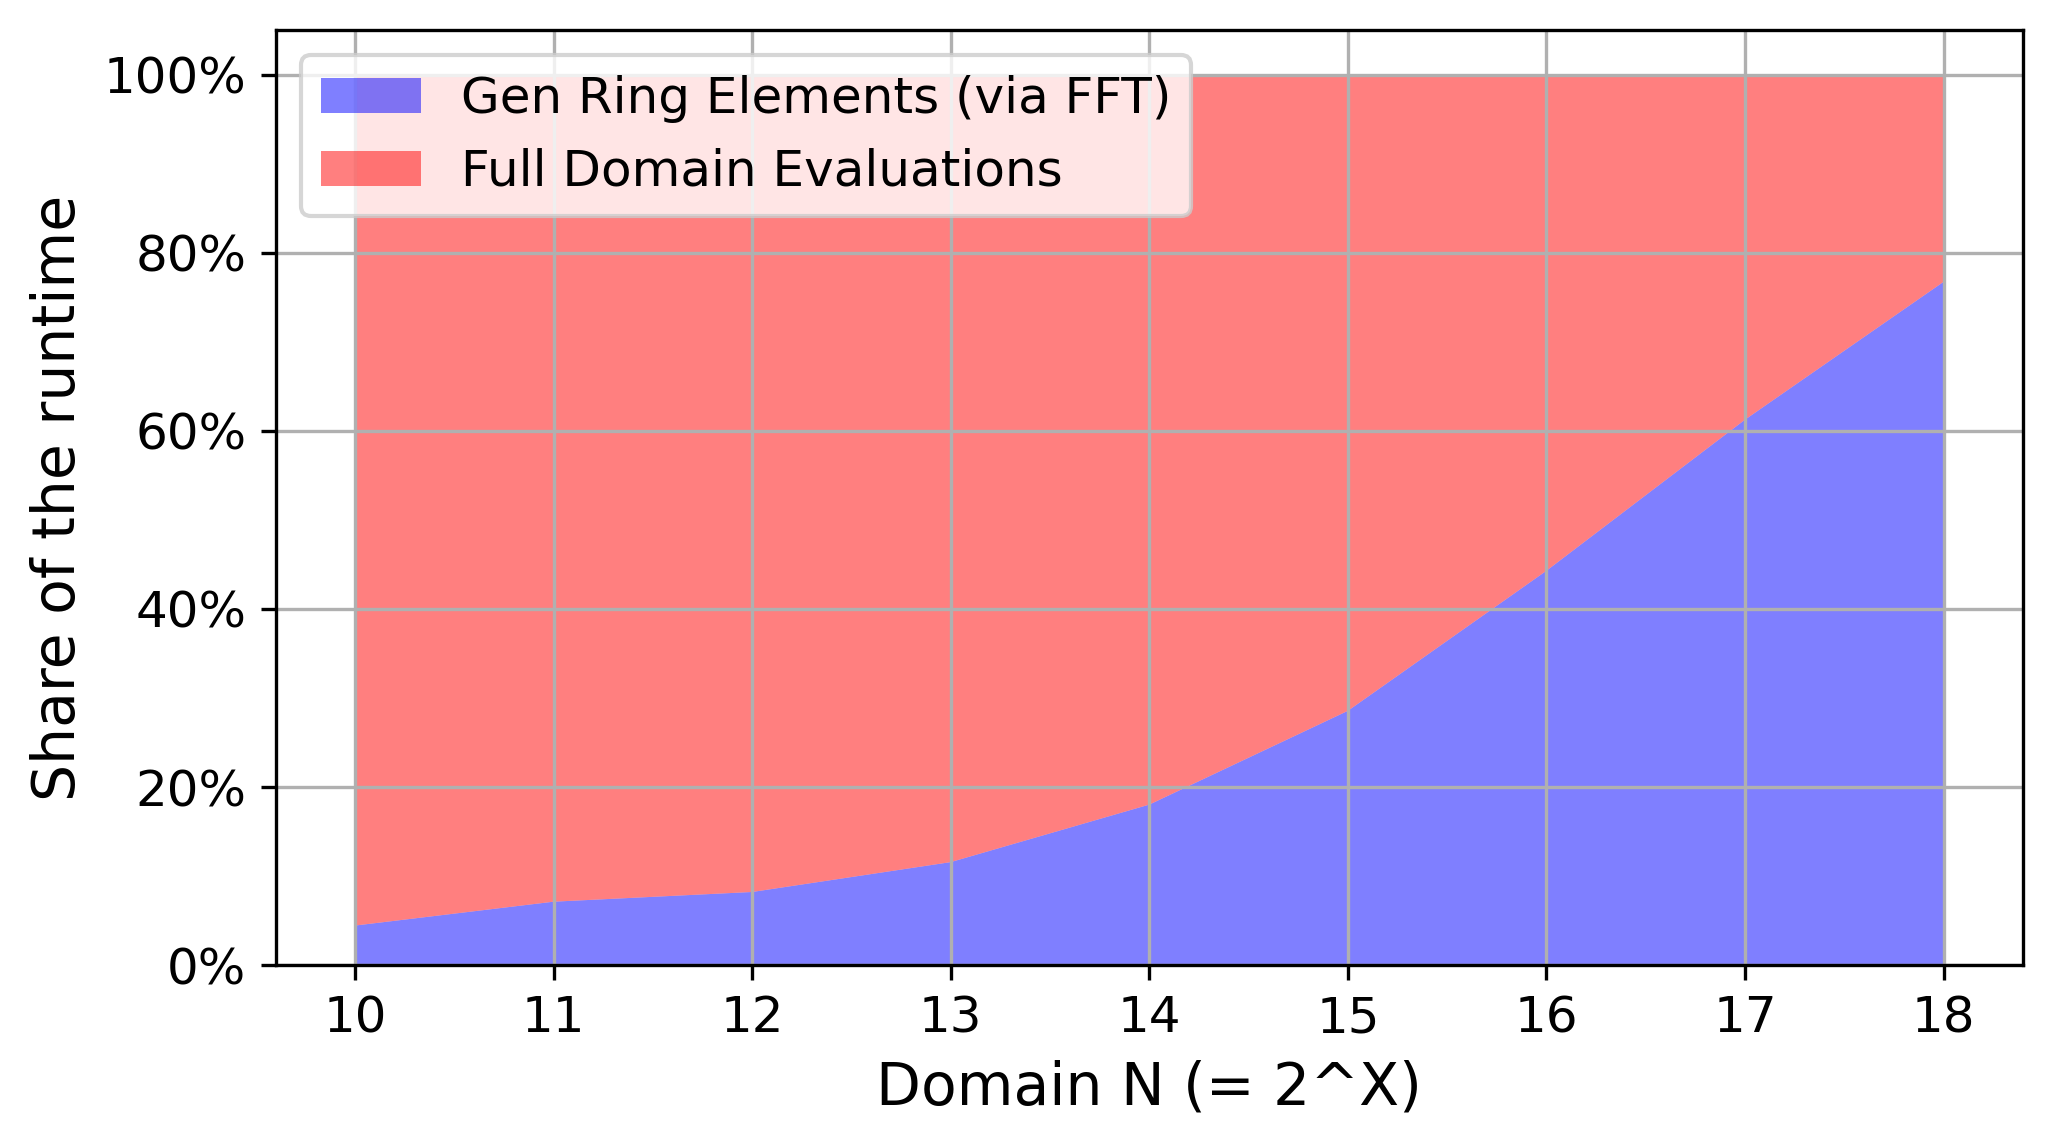
\includegraphics[scale=0.49]{images/plots/ole_percentage_dist.png}
        \caption{OLE construction}
    \end{subfigure}
    \hspace{0em}
    \begin{subfigure}[b]{0.5\textwidth}
        \centering
        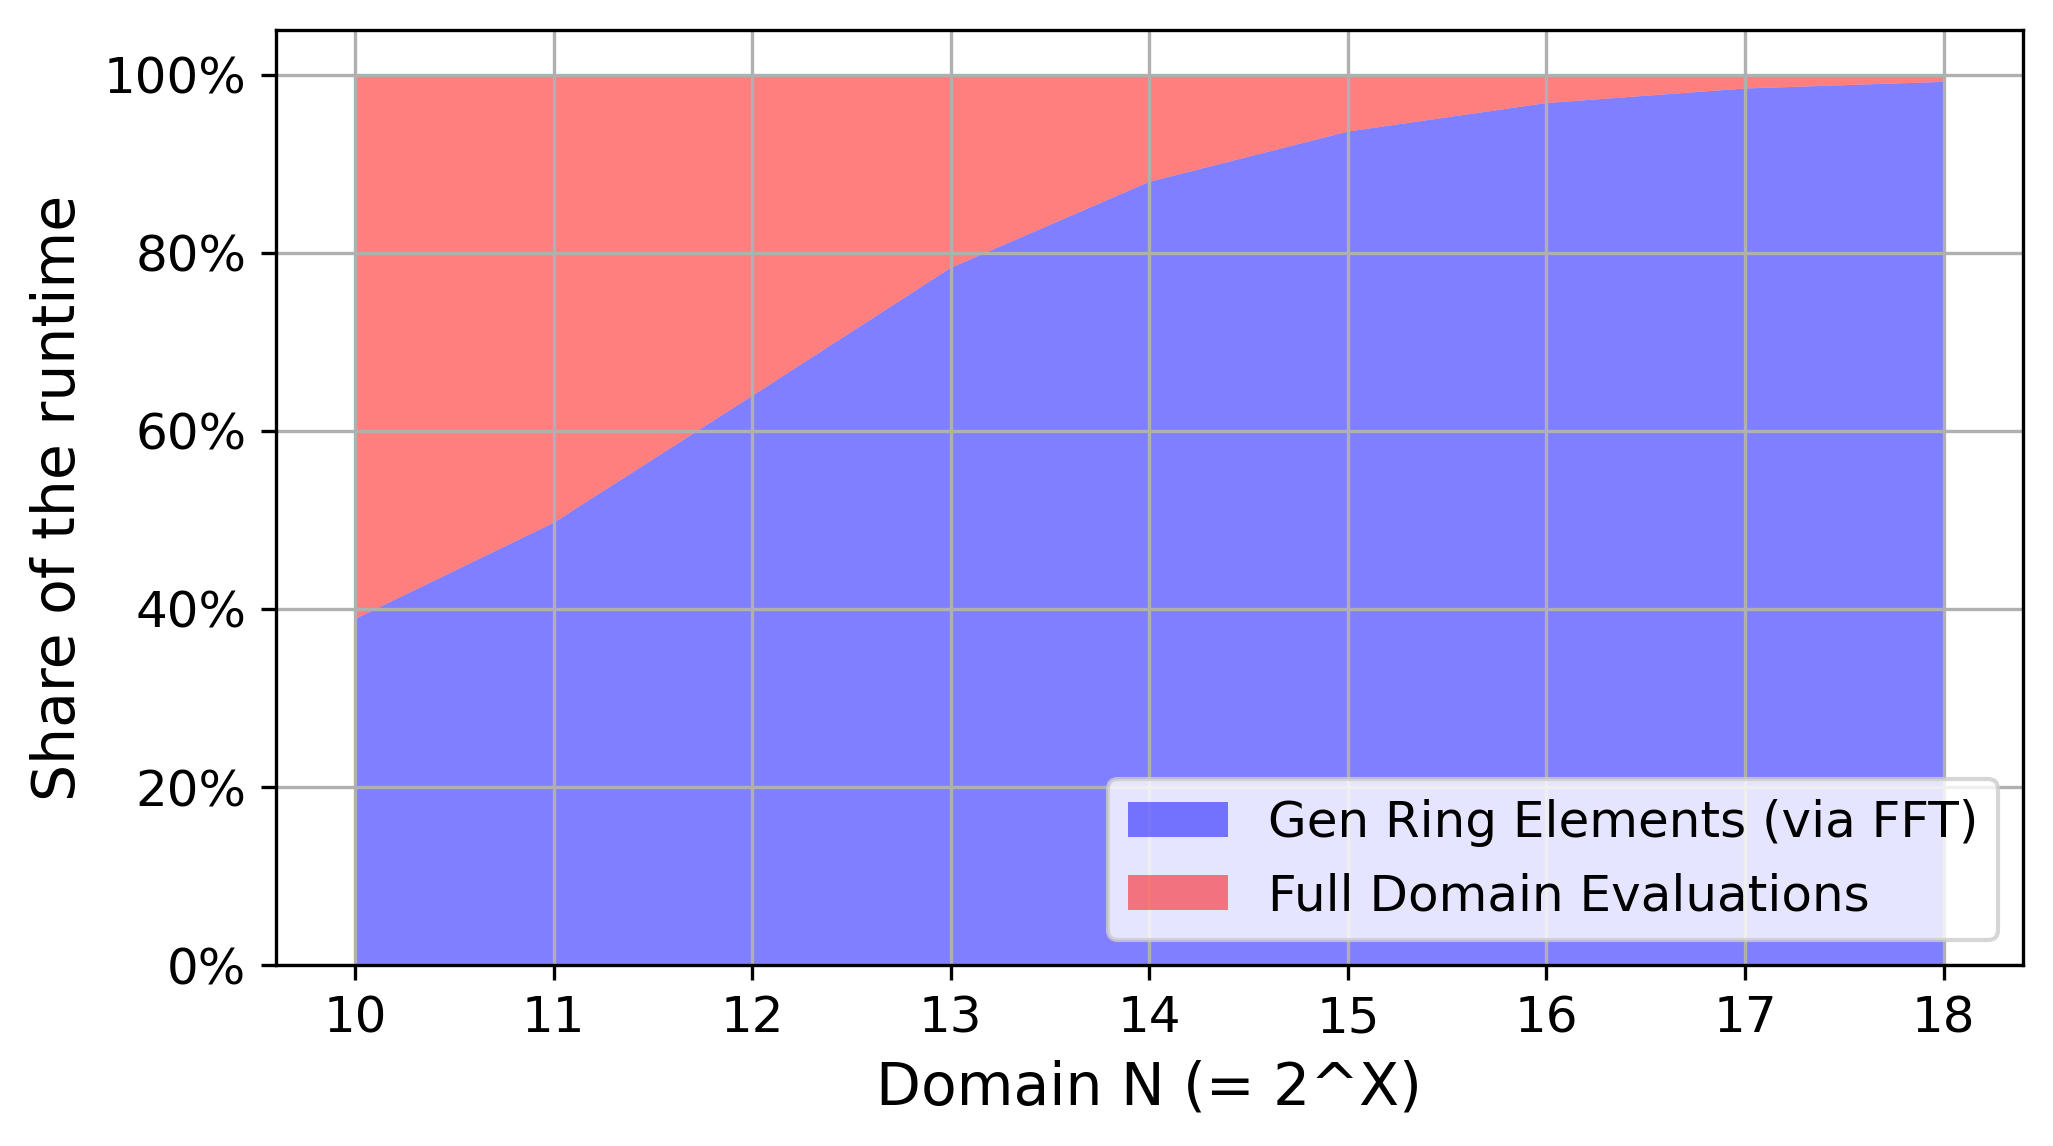
\includegraphics[scale=0.49]{images/plots/vole_percentage_dist.png}
        \caption{VOLE construction}
    \end{subfigure}
    \label{fig:runtimeAllocationComparision}
    \caption{Comparing runtime allocation of \texttt{PCG.Expand} over $N$}
\end{figure}

\textbf{Full Domain Evaluation:} Processing DSPF full domain evaluations contributes significantly to the overall runtime of the OLE case. This becomes evident when examining the following for $N=2^{17}$:
\begin{itemize}
\item OLE: Employing 16x \texttt{DSPF$^{t^2}_{2N}$.FullEval} comprises around 23\% of runtime.
\item VOLE: Utilizing 4x \texttt{DSPF$^{t}_{N}$.FullEval} accounts for only 1.5\% of runtime.  
\end{itemize}
This disparity, coupled with the higher frequency of polynomial multiplication, provides a clear explanation for the longer runtime and worse scaling of the OLE construction. Although we observe these attributes, we believe that the superlinear performance of both constructions is quite acceptable for practical applications. We provide an example of such an application in the following chapter.
